\documentclass[aspectratio=169,10pt]{beamer}
\usepackage[T1]{fontenc}
\usepackage{lmodern}
\usepackage{booktabs,pifont,array,appendixnumberbeamer}
\usepackage{tikz,pgfplots}
\usetikzlibrary{calc,plotmarks,arrows.meta,positioning}
\usepgfplotslibrary{groupplots}
\pgfplotsset{compat=1.18}

% Validated light-mode palette (categorical sets checked all-pairs; see make_figures.py).
\definecolor{cInk}{HTML}{0B0B0B}
\definecolor{cInk2}{HTML}{52514E}
\definecolor{cGrid}{HTML}{D9D8D3}
\definecolor{cNA}{HTML}{E4E3DE}
\definecolor{cTake}{HTML}{F0EFEC}
\definecolor{cBlue}{HTML}{2A78D6}
\definecolor{cOrange}{HTML}{EB6834}
\definecolor{cAqua}{HTML}{1BAF7A}
\definecolor{cViolet}{HTML}{6250D6}
\definecolor{cGreen}{HTML}{008300}
\definecolor{cMagenta}{HTML}{E87BA4}
\definecolor{sGood}{HTML}{0CA30C}
\definecolor{sWarn}{HTML}{D99400}
\definecolor{sCrit}{HTML}{D03B3B}

\setbeamertemplate{navigation symbols}{}
\setbeamercolor{normal text}{fg=cInk,bg=white}
\setbeamercolor{structure}{fg=cInk}
\setbeamercolor{frametitle}{fg=cInk}
\setbeamercolor{title}{fg=cInk}
\setbeamerfont{frametitle}{series=\bfseries,size=\large}
\setbeamersize{text margin left=0.7cm,text margin right=0.7cm}
\setbeamertemplate{frametitle}{\vspace*{0.45em}\insertframetitle\par\vspace{-0.35em}{\color{cGrid}\rule{\textwidth}{0.5pt}}}
\setbeamertemplate{footline}{\hfill{\tiny\color{cInk2}\insertframenumber\,/\,\inserttotalframenumber}\hspace*{0.6em}\vspace*{0.45em}}
\setbeamertemplate{itemize items}{\textbullet}
\setbeamertemplate{itemize subitem}{--}
\setlength{\leftmargini}{1.1em}

\newcommand{\takeaway}[1]{%
  \par\vspace{2pt}\noindent\colorbox{cTake}{\parbox{\dimexpr\textwidth-2\fboxsep\relax}{\small #1}}}
\newcommand{\src}[1]{{\par\vspace{1pt}\tiny\color{cInk2}#1\par}}
\newcommand{\yes}{\textcolor{sGood}{\ding{51}}}
\newcommand{\partly}{\textcolor{sWarn}{\textbf{$\sim$}}}
\newcommand{\no}{\textcolor{cInk2}{$\circ$}}

\title{NATO field-trial SERS dataset}
\subtitle{Progress update, results and paper options}
\author{Jesse Levine}
\institute{National Research Council Canada}
\date{Meeting with Li-Lin \,$\cdot$\, 21 October 2026}

\begin{document}

% -------------------------------------------------------------------------- 1
\begin{frame}[plain]
\titlepage
\end{frame}

% -------------------------------------------------------------------------- 2
\begin{frame}{Since we last spoke (14 September)}
\textbf{Already reported:} the classical machine-learning baseline. Extra Trees identified the chemical on an instrument it had never seen with 68.5\% balanced accuracy (chance: 33\%).

\vspace{0.6em}
\textbf{New since then}
\begin{enumerate}
  \item Compact neural networks (CNNs), including versions trained to ignore instrument differences.
  \item Three preprocessing pipelines --- minimal, smoothing, baseline correction --- tested on every model.
  \item Your question from 1 September: do the substrates detect the analyte independently of the instrument?
\end{enumerate}

\vspace{0.6em}
\textbf{For discussion}
\begin{itemize}
  \item What paper this dataset supports, and where to submit it.
  \item What a new dataset would need for the original neural-network goal.
\end{itemize}
\end{frame}

% -------------------------------------------------------------------------- 3
\begin{frame}{What we set out to do}
\begin{columns}[T,onlytextwidth]
\column{0.48\textwidth}
\textbf{Original idea}\par\smallskip
Train a disentangled variational autoencoder (VAE) to split each spectrum into a chemical part and a substrate/instrument part.

\medskip
\textbf{Why this dataset cannot support it}
\begin{itemize}
  \item No pure-analyte reference spectra, so a ``chemical part'' cannot be checked.
  \item Chemicals, substrates and instruments are not crossed: 374 of 2,760 sample $\times$ substrate $\times$ instrument combinations were measured.
  \item Only 69 independently prepared samples.
\end{itemize}
\column{0.48\textwidth}
\textbf{Current focus}\par\smallskip
Your clarification: the trial asked whether the SERS substrates detect the analyte \emph{independently of the instrument}.

\medskip
\textbf{Main question}\par\smallskip
Can a model identify the chemical on an instrument --- and on samples --- that it never saw during training?

\medskip
\textbf{Follow-up questions}\par\smallskip
When does preprocessing help? Do neural networks add anything over classical methods? Which substrates hold up across instruments?
\end{columns}
\end{frame}

% -------------------------------------------------------------------------- 4
\begin{frame}{The dataset}
\begin{columns}[T,onlytextwidth]
\column{0.37\textwidth}
\small
\begin{tabular}{@{}r@{\;\;}l@{}}
1,172 & logged recordings\\
721 & with a named SERS substrate\\
626 & pass numeric quality checks\\
615 & traceable to a sample and target\\
\textbf{598} & \textbf{unique spectra}\\
\textbf{69} & \textbf{independent physical samples}\\
\end{tabular}

\medskip
\scriptsize
\begin{tabular}{@{}lll@{}}
\toprule
Station & Chemicals & Samples\\
\midrule
CWA & 4-nitrophenol, ethanol, ethyl paraoxon & 24\\
Pills & 4-ANPP, benzyl fentanyl, blank & 20\\
Surfaces & 4-ANPP, acetaminophen, benzyl fentanyl & 25\\
\bottomrule
\end{tabular}

\medskip
Two reduced sets check the results: 500 spectra (quality-flagged removed) and 575 (Mira-1 removed; it failed its system check).
\column{0.60\textwidth}
\centering
\scriptsize\textbf{Spectra per substrate and instrument}\par\smallskip
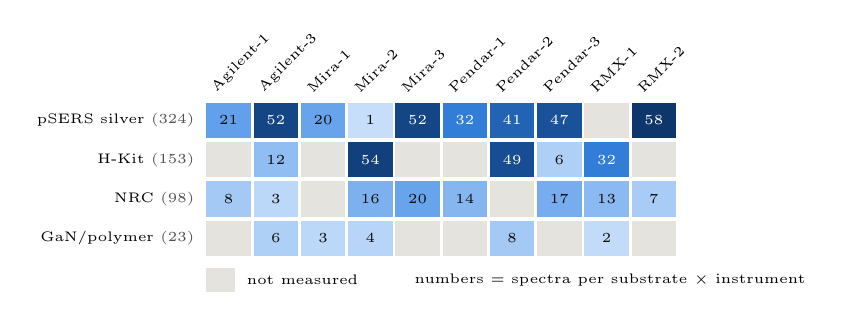
\begin{tikzpicture}[x=0.6cm,y=0.5cm,font=\tiny]
\fill[fill={rgb,255:red,98;green,160;blue,235}] (0,3) rectangle +(0.94,0.9);
\node[text=cInk] at (0.47,3.45) {21};
\fill[fill={rgb,255:red,20;green,69;blue,133}] (1,3) rectangle +(0.94,0.9);
\node[text=white] at (1.47,3.45) {52};
\fill[fill={rgb,255:red,104;green,164;blue,235}] (2,3) rectangle +(0.94,0.9);
\node[text=cInk] at (2.4699999999999998,3.45) {20};
\fill[fill={rgb,255:red,198;green,222;blue,250}] (3,3) rectangle +(0.94,0.9);
\node[text=cInk] at (3.4699999999999998,3.45) {1};
\fill[fill={rgb,255:red,20;green,69;blue,133}] (4,3) rectangle +(0.94,0.9);
\node[text=white] at (4.47,3.45) {52};
\fill[fill={rgb,255:red,50;green,125;blue,216}] (5,3) rectangle +(0.94,0.9);
\node[text=white] at (5.47,3.45) {32};
\fill[fill={rgb,255:red,34;green,99;blue,180}] (6,3) rectangle +(0.94,0.9);
\node[text=white] at (6.47,3.45) {41};
\fill[fill={rgb,255:red,26;green,82;blue,154}] (7,3) rectangle +(0.94,0.9);
\node[text=white] at (7.47,3.45) {47};
\fill[cNA] (8,3) rectangle +(0.94,0.9);
\fill[fill={rgb,255:red,13;green,54;blue,107}] (9,3) rectangle +(0.94,0.9);
\node[text=white] at (9.47,3.45) {58};
\fill[cNA] (0,2) rectangle +(0.94,0.9);
\fill[fill={rgb,255:red,144;green,189;blue,242}] (1,2) rectangle +(0.94,0.9);
\node[text=cInk] at (1.47,2.45) {12};
\fill[cNA] (2,2) rectangle +(0.94,0.9);
\fill[fill={rgb,255:red,18;green,64;blue,124}] (3,2) rectangle +(0.94,0.9);
\node[text=white] at (3.4699999999999998,2.45) {54};
\fill[cNA] (4,2) rectangle +(0.94,0.9);
\fill[cNA] (5,2) rectangle +(0.94,0.9);
\fill[fill={rgb,255:red,23;green,77;blue,146}] (6,2) rectangle +(0.94,0.9);
\node[text=white] at (6.47,2.45) {49};
\fill[fill={rgb,255:red,174;green,207;blue,246}] (7,2) rectangle +(0.94,0.9);
\node[text=cInk] at (7.47,2.45) {6};
\fill[fill={rgb,255:red,50;green,125;blue,216}] (8,2) rectangle +(0.94,0.9);
\node[text=white] at (8.47,2.45) {32};
\fill[cNA] (9,2) rectangle +(0.94,0.9);
\fill[fill={rgb,255:red,164;green,201;blue,245}] (0,1) rectangle +(0.94,0.9);
\node[text=cInk] at (0.47,1.45) {8};
\fill[fill={rgb,255:red,188;green,216;blue,248}] (1,1) rectangle +(0.94,0.9);
\node[text=cInk] at (1.47,1.45) {3};
\fill[cNA] (2,1) rectangle +(0.94,0.9);
\fill[fill={rgb,255:red,124;green,176;blue,238}] (3,1) rectangle +(0.94,0.9);
\node[text=cInk] at (3.4699999999999998,1.45) {16};
\fill[fill={rgb,255:red,104;green,164;blue,235}] (4,1) rectangle +(0.94,0.9);
\node[text=cInk] at (4.47,1.45) {20};
\fill[fill={rgb,255:red,134;green,182;blue,240}] (5,1) rectangle +(0.94,0.9);
\node[text=cInk] at (5.47,1.45) {14};
\fill[cNA] (6,1) rectangle +(0.94,0.9);
\fill[fill={rgb,255:red,119;green,173;blue,238}] (7,1) rectangle +(0.94,0.9);
\node[text=cInk] at (7.47,1.45) {17};
\fill[fill={rgb,255:red,139;green,185;blue,241}] (8,1) rectangle +(0.94,0.9);
\node[text=cInk] at (8.47,1.45) {13};
\fill[fill={rgb,255:red,169;green,204;blue,246}] (9,1) rectangle +(0.94,0.9);
\node[text=cInk] at (9.47,1.45) {7};
\fill[cNA] (0,0) rectangle +(0.94,0.9);
\fill[fill={rgb,255:red,174;green,207;blue,246}] (1,0) rectangle +(0.94,0.9);
\node[text=cInk] at (1.47,0.45) {6};
\fill[fill={rgb,255:red,188;green,216;blue,248}] (2,0) rectangle +(0.94,0.9);
\node[text=cInk] at (2.4699999999999998,0.45) {3};
\fill[fill={rgb,255:red,183;green,213;blue,248}] (3,0) rectangle +(0.94,0.9);
\node[text=cInk] at (3.4699999999999998,0.45) {4};
\fill[cNA] (4,0) rectangle +(0.94,0.9);
\fill[cNA] (5,0) rectangle +(0.94,0.9);
\fill[fill={rgb,255:red,164;green,201;blue,245}] (6,0) rectangle +(0.94,0.9);
\node[text=cInk] at (6.47,0.45) {8};
\fill[cNA] (7,0) rectangle +(0.94,0.9);
\fill[fill={rgb,255:red,193;green,219;blue,249}] (8,0) rectangle +(0.94,0.9);
\node[text=cInk] at (8.47,0.45) {2};
\fill[cNA] (9,0) rectangle +(0.94,0.9);
\node[rotate=45,anchor=south west,inner sep=1pt] at (0.25,4.0) {Agilent-1};
\node[rotate=45,anchor=south west,inner sep=1pt] at (1.25,4.0) {Agilent-3};
\node[rotate=45,anchor=south west,inner sep=1pt] at (2.25,4.0) {Mira-1};
\node[rotate=45,anchor=south west,inner sep=1pt] at (3.25,4.0) {Mira-2};
\node[rotate=45,anchor=south west,inner sep=1pt] at (4.25,4.0) {Mira-3};
\node[rotate=45,anchor=south west,inner sep=1pt] at (5.25,4.0) {Pendar-1};
\node[rotate=45,anchor=south west,inner sep=1pt] at (6.25,4.0) {Pendar-2};
\node[rotate=45,anchor=south west,inner sep=1pt] at (7.25,4.0) {Pendar-3};
\node[rotate=45,anchor=south west,inner sep=1pt] at (8.25,4.0) {RMX-1};
\node[rotate=45,anchor=south west,inner sep=1pt] at (9.25,4.0) {RMX-2};
\node[anchor=east] at (-0.05,3.45) {pSERS silver \textcolor{cInk2}{(324)}};
\node[anchor=east] at (-0.05,2.45) {H-Kit \textcolor{cInk2}{(153)}};
\node[anchor=east] at (-0.05,1.45) {NRC \textcolor{cInk2}{(98)}};
\node[anchor=east] at (-0.05,0.45) {GaN/polymer \textcolor{cInk2}{(23)}};
\fill[cNA] (0,-0.9) rectangle +(0.6,0.6); \node[anchor=west] at (0.65,-0.6) {not measured};
\node[anchor=west] at (4.2,-0.6) {numbers = spectra per substrate $\times$ instrument};
\end{tikzpicture}

\end{columns}
\takeaway{The 598 spectra are repeat views of 69 samples. Every test keeps all views of one sample on the same side of the train/test split.}
\end{frame}

% -------------------------------------------------------------------------- 5
\begin{frame}{Instrument differences dominate the raw spectra}
\begin{columns}[c,onlytextwidth]
\column{0.64\textwidth}
\centering
\input{figures/pca_pills.tex}
\column{0.34\textwidth}
\small
Pills station: principal-component map of 208 spectra (one point per spectrum).

\medskip
\textbf{Minimal preprocessing:} a spectrum's nearest neighbour from another sample has the same instrument brand 95\% of the time, but the same chemical only 43\%. Both would be about 1 in 3 by chance.

\medskip
\textbf{Baseline correction} weakens the brand grouping (59\% brand, 52\% chemical). At Surfaces it reverses: 42\% brand, 74\% chemical.
\end{columns}
\takeaway{Removing the background moves spectra from grouping by instrument toward grouping by chemical. It does not remove the instrument effect completely.}
\end{frame}

% -------------------------------------------------------------------------- 6
\begin{frame}{Seven questions and where each stands}
\small
\renewcommand{\arraystretch}{1.25}
\begin{tabular}{@{}c@{\;}>{\raggedright\arraybackslash}p{0.45\textwidth}>{\raggedright\arraybackslash}p{0.47\textwidth}@{}}
\toprule
& Question & Status\\
\midrule
\yes & 1. Identify the chemical on an unseen instrument? & 65--68\% minimal; 70--75\% baseline-corrected (chance 33\%)\\
\yes & 2. Which single preprocessing pipeline helps most? & Baseline correction: +5 to +7 points; smoothing: no gain\\
\partly & 3. Should preprocessing adapt to the instrument? & By brand: not testable here. By spectrum quality: possible at CWA only; not yet run\\
\yes & 4. Do neural networks beat classical methods? & No clear difference\\
\no & 5. How much do 1--2 calibration samples from a new instrument help? & Not yet run; feasible for 1--2 samples per chemical\\
\no & 6. Are confidence scores reliable; can unknowns be flagged? & Not yet run; CNN confidence is poorly calibrated\\
\partly & 7. Do substrates work independently of the instrument? & Partly: depends on the instrument; Mira units are the weakest\\
\bottomrule
\end{tabular}

\src{\yes\ answered \quad \partly\ partly answered \quad \no\ not yet run. Balanced accuracy averages the hit rate over chemicals, so 33\% is chance for three chemicals.}
\end{frame}

% -------------------------------------------------------------------------- 7
\begin{frame}{Results: identifying chemicals on an unseen instrument}
\begin{columns}[T,onlytextwidth]
\column{0.52\textwidth}
\centering
\scriptsize\textbf{Five models $\times$ three preprocessing pipelines}\par\smallskip
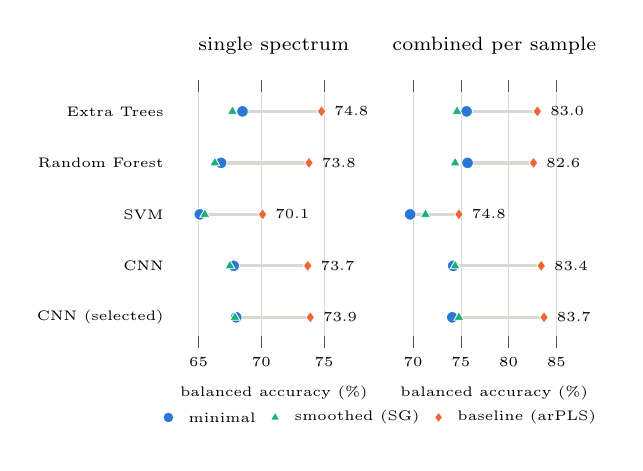
\begin{tikzpicture}
\begin{groupplot}[group style={group size=2 by 1,horizontal sep=0.25cm,yticklabels at=edge left},
  width=2.55cm,height=3.4cm,scale only axis,ymin=0.4,ymax=5.6,
  ytick={5,4,3,2,1},yticklabels={{Extra Trees},{Random Forest},{SVM},{CNN},{CNN (selected)}},
  tick label style={font=\tiny},title style={font=\scriptsize},xlabel style={font=\tiny},
  xmajorgrids,grid style={cGrid,very thin},axis line style={cInk2},tick style={cInk2},
  y axis line style={draw=none},ytick style={draw=none}]
\nextgroupplot[title={single spectrum},xmin=63,xmax=79,xlabel={balanced accuracy (\%)}]
\draw[cGrid,line width=1.2pt] (axis cs:68.5,5) -- (axis cs:74.8,5);
\draw[cGrid,line width=1.2pt] (axis cs:66.8,4) -- (axis cs:73.8,4);
\draw[cGrid,line width=1.2pt] (axis cs:65.1,3) -- (axis cs:70.1,3);
\draw[cGrid,line width=1.2pt] (axis cs:67.8,2) -- (axis cs:73.7,2);
\draw[cGrid,line width=1.2pt] (axis cs:68.0,1) -- (axis cs:73.9,1);
\addplot[only marks,mark=*,mark size=2.1pt,color=cBlue,mark options={fill=cBlue,draw=white,line width=0.3pt}] coordinates {(68.5,5) (66.8,4) (65.1,3) (67.8,2) (68.0,1)};
\addplot[only marks,mark=triangle*,mark size=2.1pt,color=cAqua,mark options={fill=cAqua,draw=white,line width=0.3pt}] coordinates {(67.7,5) (66.3,4) (65.5,3) (67.5,2) (67.9,1)};
\addplot[only marks,mark=diamond*,mark size=2.1pt,color=cOrange,mark options={fill=cOrange,draw=white,line width=0.3pt}] coordinates {(74.8,5) (73.8,4) (70.1,3) (73.7,2) (73.9,1)};
\node[font=\tiny,anchor=west,text=cInk] at (axis cs:74.8,5) {\,74.8};
\node[font=\tiny,anchor=west,text=cInk] at (axis cs:73.8,4) {\,73.8};
\node[font=\tiny,anchor=west,text=cInk] at (axis cs:70.1,3) {\,70.1};
\node[font=\tiny,anchor=west,text=cInk] at (axis cs:73.7,2) {\,73.7};
\node[font=\tiny,anchor=west,text=cInk] at (axis cs:73.9,1) {\,73.9};
\nextgroupplot[title={combined per sample},xmin=68,xmax=89,xlabel={balanced accuracy (\%)}]
\draw[cGrid,line width=1.2pt] (axis cs:75.6,5) -- (axis cs:83.0,5);
\draw[cGrid,line width=1.2pt] (axis cs:75.7,4) -- (axis cs:82.6,4);
\draw[cGrid,line width=1.2pt] (axis cs:69.7,3) -- (axis cs:74.8,3);
\draw[cGrid,line width=1.2pt] (axis cs:74.2,2) -- (axis cs:83.4,2);
\draw[cGrid,line width=1.2pt] (axis cs:74.1,1) -- (axis cs:83.7,1);
\addplot[only marks,mark=*,mark size=2.1pt,color=cBlue,mark options={fill=cBlue,draw=white,line width=0.3pt}] coordinates {(75.6,5) (75.7,4) (69.7,3) (74.2,2) (74.1,1)};
\addplot[only marks,mark=triangle*,mark size=2.1pt,color=cAqua,mark options={fill=cAqua,draw=white,line width=0.3pt}] coordinates {(74.6,5) (74.4,4) (71.3,3) (74.4,2) (74.8,1)};
\addplot[only marks,mark=diamond*,mark size=2.1pt,color=cOrange,mark options={fill=cOrange,draw=white,line width=0.3pt}] coordinates {(83.0,5) (82.6,4) (74.8,3) (83.4,2) (83.7,1)};
\node[font=\tiny,anchor=west,text=cInk] at (axis cs:83.0,5) {\,83.0};
\node[font=\tiny,anchor=west,text=cInk] at (axis cs:82.6,4) {\,82.6};
\node[font=\tiny,anchor=west,text=cInk] at (axis cs:74.8,3) {\,74.8};
\node[font=\tiny,anchor=west,text=cInk] at (axis cs:83.4,2) {\,83.4};
\node[font=\tiny,anchor=west,text=cInk] at (axis cs:83.7,1) {\,83.7};
\end{groupplot}
\matrix[anchor=north,font=\tiny,column sep=2pt] at ($(group c1r1.south)!0.5!(group c2r1.south)+(0,-0.55)$) {\draw[fill=cBlue,draw=white] plot[mark=*,mark size=2pt] coordinates {(0,0)}; & \node[anchor=west]{minimal}; &\draw[fill=cAqua,draw=white] plot[mark=triangle*,mark size=2pt] coordinates {(0,0)}; & \node[anchor=west]{smoothed (SG)}; &\draw[fill=cOrange,draw=white] plot[mark=diamond*,mark size=2pt] coordinates {(0,0)}; & \node[anchor=west]{baseline (arPLS)}; \\};
\end{tikzpicture}

\column{0.46\textwidth}
\centering
\scriptsize\textbf{Which chemicals are confused}\par\smallskip
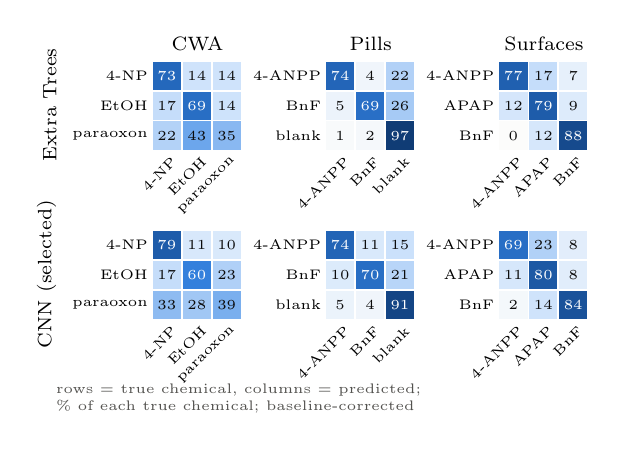
\begin{tikzpicture}[font=\tiny]
\fill[fill={rgb,255:red,36;green,104;blue,188}] (0.950,2.910) rectangle +(0.361,0.361);
\node[text=white] at (1.131,3.091) {73};
\fill[fill={rgb,255:red,207;green,227;blue,251}] (1.330,2.910) rectangle +(0.361,0.361);
\node[text=cInk] at (1.510,3.091) {14};
\fill[fill={rgb,255:red,207;green,227;blue,251}] (1.710,2.910) rectangle +(0.361,0.361);
\node[text=cInk] at (1.890,3.091) {14};
\fill[fill={rgb,255:red,197;green,221;blue,250}] (0.950,2.530) rectangle +(0.361,0.361);
\node[text=cInk] at (1.131,2.710) {17};
\fill[fill={rgb,255:red,40;green,110;blue,196}] (1.330,2.530) rectangle +(0.361,0.361);
\node[text=white] at (1.510,2.710) {69};
\fill[fill={rgb,255:red,206;green,227;blue,251}] (1.710,2.530) rectangle +(0.361,0.361);
\node[text=cInk] at (1.890,2.710) {14};
\fill[fill={rgb,255:red,179;green,210;blue,247}] (0.950,2.150) rectangle +(0.361,0.361);
\node[text=cInk] at (1.131,2.330) {22};
\fill[fill={rgb,255:red,108;green,166;blue,236}] (1.330,2.150) rectangle +(0.361,0.361);
\node[text=cInk] at (1.510,2.330) {43};
\fill[fill={rgb,255:red,137;green,184;blue,241}] (1.710,2.150) rectangle +(0.361,0.361);
\node[text=cInk] at (1.890,2.330) {35};
\node[anchor=east,inner sep=1pt] at (0.930,3.091) {4-NP};
\node[anchor=north east,rotate=45,inner sep=1pt] at (1.178,2.130) {4-NP};
\node[anchor=east,inner sep=1pt] at (0.930,2.710) {EtOH};
\node[anchor=north east,rotate=45,inner sep=1pt] at (1.558,2.130) {EtOH};
\node[anchor=east,inner sep=1pt] at (0.930,2.330) {paraoxon};
\node[anchor=north east,rotate=45,inner sep=1pt] at (1.938,2.130) {paraoxon};
\node[anchor=south,font=\scriptsize] at (1.520,3.290) {CWA};
\fill[fill={rgb,255:red,35;green,101;blue,184}] (3.150,2.910) rectangle +(0.361,0.361);
\node[text=white] at (3.331,3.091) {74};
\fill[fill={rgb,255:red,240;green,245;blue,251}] (3.530,2.910) rectangle +(0.361,0.361);
\node[text=cInk] at (3.711,3.091) {4};
\fill[fill={rgb,255:red,178;green,209;blue,247}] (3.910,2.910) rectangle +(0.361,0.361);
\node[text=cInk] at (4.091,3.091) {22};
\fill[fill={rgb,255:red,236;green,243;blue,251}] (3.150,2.530) rectangle +(0.361,0.361);
\node[text=cInk] at (3.331,2.710) {5};
\fill[fill={rgb,255:red,41;green,111;blue,198}] (3.530,2.530) rectangle +(0.361,0.361);
\node[text=white] at (3.711,2.710) {69};
\fill[fill={rgb,255:red,166;green,202;blue,245}] (3.910,2.530) rectangle +(0.361,0.361);
\node[text=cInk] at (4.091,2.710) {26};
\fill[fill={rgb,255:red,248;green,250;blue,251}] (3.150,2.150) rectangle +(0.361,0.361);
\node[text=cInk] at (3.331,2.330) {1};
\fill[fill={rgb,255:red,245;green,248;blue,251}] (3.530,2.150) rectangle +(0.361,0.361);
\node[text=cInk] at (3.711,2.330) {2};
\fill[fill={rgb,255:red,16;green,60;blue,117}] (3.910,2.150) rectangle +(0.361,0.361);
\node[text=white] at (4.091,2.330) {97};
\node[anchor=east,inner sep=1pt] at (3.130,3.091) {4-ANPP};
\node[anchor=north east,rotate=45,inner sep=1pt] at (3.378,2.130) {4-ANPP};
\node[anchor=east,inner sep=1pt] at (3.130,2.710) {BnF};
\node[anchor=north east,rotate=45,inner sep=1pt] at (3.758,2.130) {BnF};
\node[anchor=east,inner sep=1pt] at (3.130,2.330) {blank};
\node[anchor=north east,rotate=45,inner sep=1pt] at (4.138,2.130) {blank};
\node[anchor=south,font=\scriptsize] at (3.720,3.290) {Pills};
\fill[fill={rgb,255:red,32;green,96;blue,176}] (5.350,2.910) rectangle +(0.361,0.361);
\node[text=white] at (5.531,3.091) {77};
\fill[fill={rgb,255:red,197;green,221;blue,250}] (5.730,2.910) rectangle +(0.361,0.361);
\node[text=cInk] at (5.911,3.091) {17};
\fill[fill={rgb,255:red,230;green,240;blue,251}] (6.110,2.910) rectangle +(0.361,0.361);
\node[text=cInk] at (6.291,3.091) {7};
\fill[fill={rgb,255:red,213;green,230;blue,251}] (5.350,2.530) rectangle +(0.361,0.361);
\node[text=cInk] at (5.531,2.710) {12};
\fill[fill={rgb,255:red,30;green,92;blue,170}] (5.730,2.530) rectangle +(0.361,0.361);
\node[text=white] at (5.911,2.710) {79};
\fill[fill={rgb,255:red,221;green,235;blue,251}] (6.110,2.530) rectangle +(0.361,0.361);
\node[text=cInk] at (6.291,2.710) {9};
\fill[fill={rgb,255:red,252;green,252;blue,251}] (5.350,2.150) rectangle +(0.361,0.361);
\node[text=cInk] at (5.531,2.330) {0};
\fill[fill={rgb,255:red,214;green,231;blue,251}] (5.730,2.150) rectangle +(0.361,0.361);
\node[text=cInk] at (5.911,2.330) {12};
\fill[fill={rgb,255:red,22;green,74;blue,141}] (6.110,2.150) rectangle +(0.361,0.361);
\node[text=white] at (6.291,2.330) {88};
\node[anchor=east,inner sep=1pt] at (5.330,3.091) {4-ANPP};
\node[anchor=north east,rotate=45,inner sep=1pt] at (5.578,2.130) {4-ANPP};
\node[anchor=east,inner sep=1pt] at (5.330,2.710) {APAP};
\node[anchor=north east,rotate=45,inner sep=1pt] at (5.958,2.130) {APAP};
\node[anchor=east,inner sep=1pt] at (5.330,2.330) {BnF};
\node[anchor=north east,rotate=45,inner sep=1pt] at (6.338,2.130) {BnF};
\node[anchor=south,font=\scriptsize] at (5.920,3.290) {Surfaces};
\node[rotate=90,anchor=south,font=\scriptsize] at (-0.15,2.720) {Extra Trees};
\fill[fill={rgb,255:red,30;green,92;blue,170}] (0.950,0.760) rectangle +(0.361,0.361);
\node[text=white] at (1.131,0.941) {79};
\fill[fill={rgb,255:red,216;green,232;blue,251}] (1.330,0.760) rectangle +(0.361,0.361);
\node[text=cInk] at (1.510,0.941) {11};
\fill[fill={rgb,255:red,217;green,233;blue,251}] (1.710,0.760) rectangle +(0.361,0.361);
\node[text=cInk] at (1.890,0.941) {10};
\fill[fill={rgb,255:red,197;green,221;blue,250}] (0.950,0.380) rectangle +(0.361,0.361);
\node[text=cInk] at (1.131,0.560) {17};
\fill[fill={rgb,255:red,52;green,128;blue,220}] (1.330,0.380) rectangle +(0.361,0.361);
\node[text=white] at (1.510,0.560) {60};
\fill[fill={rgb,255:red,176;green,208;blue,247}] (1.710,0.380) rectangle +(0.361,0.361);
\node[text=cInk] at (1.890,0.560) {23};
\fill[fill={rgb,255:red,142;green,187;blue,241}] (0.950,0.000) rectangle +(0.361,0.361);
\node[text=cInk] at (1.131,0.180) {33};
\fill[fill={rgb,255:red,161;green,199;blue,244}] (1.330,0.000) rectangle +(0.361,0.361);
\node[text=cInk] at (1.510,0.180) {28};
\fill[fill={rgb,255:red,122;green,175;blue,238}] (1.710,0.000) rectangle +(0.361,0.361);
\node[text=cInk] at (1.890,0.180) {39};
\node[anchor=east,inner sep=1pt] at (0.930,0.941) {4-NP};
\node[anchor=north east,rotate=45,inner sep=1pt] at (1.178,-0.020) {4-NP};
\node[anchor=east,inner sep=1pt] at (0.930,0.560) {EtOH};
\node[anchor=north east,rotate=45,inner sep=1pt] at (1.558,-0.020) {EtOH};
\node[anchor=east,inner sep=1pt] at (0.930,0.180) {paraoxon};
\node[anchor=north east,rotate=45,inner sep=1pt] at (1.938,-0.020) {paraoxon};
\fill[fill={rgb,255:red,34;green,100;blue,182}] (3.150,0.760) rectangle +(0.361,0.361);
\node[text=white] at (3.331,0.941) {74};
\fill[fill={rgb,255:red,217;green,233;blue,251}] (3.530,0.760) rectangle +(0.361,0.361);
\node[text=cInk] at (3.711,0.941) {11};
\fill[fill={rgb,255:red,203;green,225;blue,251}] (3.910,0.760) rectangle +(0.361,0.361);
\node[text=cInk] at (4.091,0.941) {15};
\fill[fill={rgb,255:red,220;green,235;blue,251}] (3.150,0.380) rectangle +(0.361,0.361);
\node[text=cInk] at (3.331,0.560) {10};
\fill[fill={rgb,255:red,40;green,110;blue,196}] (3.530,0.380) rectangle +(0.361,0.361);
\node[text=white] at (3.711,0.560) {70};
\fill[fill={rgb,255:red,184;green,213;blue,248}] (3.910,0.380) rectangle +(0.361,0.361);
\node[text=cInk] at (4.091,0.560) {21};
\fill[fill={rgb,255:red,235;green,243;blue,251}] (3.150,0.000) rectangle +(0.361,0.361);
\node[text=cInk] at (3.331,0.180) {5};
\fill[fill={rgb,255:red,240;green,245;blue,251}] (3.530,0.000) rectangle +(0.361,0.361);
\node[text=cInk] at (3.711,0.180) {4};
\fill[fill={rgb,255:red,20;green,69;blue,133}] (3.910,0.000) rectangle +(0.361,0.361);
\node[text=white] at (4.091,0.180) {91};
\node[anchor=east,inner sep=1pt] at (3.130,0.941) {4-ANPP};
\node[anchor=north east,rotate=45,inner sep=1pt] at (3.378,-0.020) {4-ANPP};
\node[anchor=east,inner sep=1pt] at (3.130,0.560) {BnF};
\node[anchor=north east,rotate=45,inner sep=1pt] at (3.758,-0.020) {BnF};
\node[anchor=east,inner sep=1pt] at (3.130,0.180) {blank};
\node[anchor=north east,rotate=45,inner sep=1pt] at (4.138,-0.020) {blank};
\fill[fill={rgb,255:red,40;green,110;blue,197}] (5.350,0.760) rectangle +(0.361,0.361);
\node[text=white] at (5.531,0.941) {69};
\fill[fill={rgb,255:red,177;green,209;blue,247}] (5.730,0.760) rectangle +(0.361,0.361);
\node[text=cInk] at (5.911,0.941) {23};
\fill[fill={rgb,255:red,226;green,237;blue,251}] (6.110,0.760) rectangle +(0.361,0.361);
\node[text=cInk] at (6.291,0.941) {8};
\fill[fill={rgb,255:red,214;green,231;blue,251}] (5.350,0.380) rectangle +(0.361,0.361);
\node[text=cInk] at (5.531,0.560) {11};
\fill[fill={rgb,255:red,29;green,89;blue,164}] (5.730,0.380) rectangle +(0.361,0.361);
\node[text=white] at (5.911,0.560) {80};
\fill[fill={rgb,255:red,225;green,237;blue,251}] (6.110,0.380) rectangle +(0.361,0.361);
\node[text=cInk] at (6.291,0.560) {8};
\fill[fill={rgb,255:red,244;green,248;blue,251}] (5.350,0.000) rectangle +(0.361,0.361);
\node[text=cInk] at (5.531,0.180) {2};
\fill[fill={rgb,255:red,207;green,227;blue,251}] (5.730,0.000) rectangle +(0.361,0.361);
\node[text=cInk] at (5.911,0.180) {14};
\fill[fill={rgb,255:red,26;green,82;blue,154}] (6.110,0.000) rectangle +(0.361,0.361);
\node[text=white] at (6.291,0.180) {84};
\node[anchor=east,inner sep=1pt] at (5.330,0.941) {4-ANPP};
\node[anchor=north east,rotate=45,inner sep=1pt] at (5.578,-0.020) {4-ANPP};
\node[anchor=east,inner sep=1pt] at (5.330,0.560) {APAP};
\node[anchor=north east,rotate=45,inner sep=1pt] at (5.958,-0.020) {APAP};
\node[anchor=east,inner sep=1pt] at (5.330,0.180) {BnF};
\node[anchor=north east,rotate=45,inner sep=1pt] at (6.338,-0.020) {BnF};
\node[rotate=90,anchor=south,font=\scriptsize] at (-0.15,0.570) {CNN (selected)};
\node[anchor=north west,text=cInk2,align=left] at (-0.4,-0.7) {rows = true chemical, columns = predicted;\\\% of each true chemical; baseline-corrected};
\end{tikzpicture}

\end{columns}
\takeaway{Baseline correction helps every model; tree models and CNNs perform alike. With minimal preprocessing, Extra Trees calls 42--45\% of Pills drug spectra ``blank''; correction roughly halves this. Ethyl paraoxon is the hardest chemical (35--39\% correct).}
\src{``Combined per sample'' averages the model's probabilities over a sample's repeat spectra (spectra are not averaged). 4-NP = 4-nitrophenol, EtOH = ethanol, BnF = benzyl fentanyl, APAP = acetaminophen.}
\end{frame}

% -------------------------------------------------------------------------- 8
\begin{frame}{Results: where it works and where it does not}
\begin{columns}[T,onlytextwidth]
\column{0.33\textwidth}
\centering
\scriptsize\textbf{Per chemical, all models (\% correct)}\par\smallskip
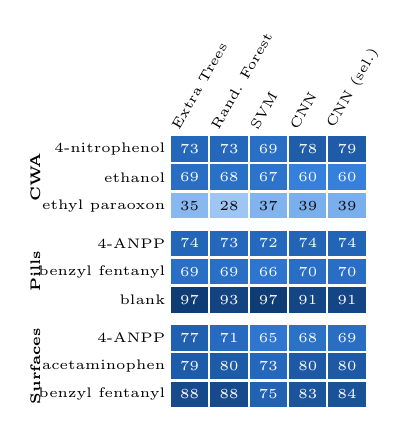
\begin{tikzpicture}[font=\tiny]
\fill[fill={rgb,255:red,36;green,104;blue,188}] (0.000,2.880) rectangle +(0.475,0.324);
\node[text=white] at (0.237,3.042) {73};
\fill[fill={rgb,255:red,36;green,103;blue,187}] (0.500,2.880) rectangle +(0.475,0.324);
\node[text=white] at (0.738,3.042) {73};
\fill[fill={rgb,255:red,40;green,111;blue,197}] (1.000,2.880) rectangle +(0.475,0.324);
\node[text=white] at (1.238,3.042) {69};
\fill[fill={rgb,255:red,31;green,93;blue,171}] (1.500,2.880) rectangle +(0.475,0.324);
\node[text=white] at (1.738,3.042) {78};
\fill[fill={rgb,255:red,30;green,92;blue,170}] (2.000,2.880) rectangle +(0.475,0.324);
\node[text=white] at (2.237,3.042) {79};
\node[anchor=east,inner sep=1pt] at (-0.03,3.042) {4-nitrophenol};
\fill[fill={rgb,255:red,40;green,110;blue,196}] (0.000,2.520) rectangle +(0.475,0.324);
\node[text=white] at (0.237,2.682) {69};
\fill[fill={rgb,255:red,41;green,112;blue,199}] (0.500,2.520) rectangle +(0.475,0.324);
\node[text=white] at (0.738,2.682) {68};
\fill[fill={rgb,255:red,43;green,115;blue,203}] (1.000,2.520) rectangle +(0.475,0.324);
\node[text=white] at (1.238,2.682) {67};
\fill[fill={rgb,255:red,52;green,128;blue,220}] (1.500,2.520) rectangle +(0.475,0.324);
\node[text=white] at (1.738,2.682) {60};
\fill[fill={rgb,255:red,52;green,128;blue,220}] (2.000,2.520) rectangle +(0.475,0.324);
\node[text=white] at (2.237,2.682) {60};
\node[anchor=east,inner sep=1pt] at (-0.03,2.682) {ethanol};
\node[rotate=90,anchor=south,font=\tiny\bfseries,inner sep=1pt] at (-1.62,2.682) {CWA};
\fill[fill={rgb,255:red,137;green,184;blue,241}] (0.000,2.160) rectangle +(0.475,0.324);
\node[text=cInk] at (0.237,2.322) {35};
\fill[fill={rgb,255:red,159;green,197;blue,244}] (0.500,2.160) rectangle +(0.475,0.324);
\node[text=cInk] at (0.738,2.322) {28};
\fill[fill={rgb,255:red,129;green,180;blue,239}] (1.000,2.160) rectangle +(0.475,0.324);
\node[text=cInk] at (1.238,2.322) {37};
\fill[fill={rgb,255:red,122;green,175;blue,238}] (1.500,2.160) rectangle +(0.475,0.324);
\node[text=cInk] at (1.738,2.322) {39};
\fill[fill={rgb,255:red,122;green,175;blue,238}] (2.000,2.160) rectangle +(0.475,0.324);
\node[text=cInk] at (2.237,2.322) {39};
\node[anchor=east,inner sep=1pt] at (-0.03,2.322) {ethyl paraoxon};
\fill[fill={rgb,255:red,35;green,101;blue,184}] (0.000,1.680) rectangle +(0.475,0.324);
\node[text=white] at (0.237,1.842) {74};
\fill[fill={rgb,255:red,36;green,103;blue,187}] (0.500,1.680) rectangle +(0.475,0.324);
\node[text=white] at (0.738,1.842) {73};
\fill[fill={rgb,255:red,36;green,105;blue,189}] (1.000,1.680) rectangle +(0.475,0.324);
\node[text=white] at (1.238,1.842) {72};
\fill[fill={rgb,255:red,34;green,100;blue,182}] (1.500,1.680) rectangle +(0.475,0.324);
\node[text=white] at (1.738,1.842) {74};
\fill[fill={rgb,255:red,34;green,100;blue,182}] (2.000,1.680) rectangle +(0.475,0.324);
\node[text=white] at (2.237,1.842) {74};
\node[anchor=east,inner sep=1pt] at (-0.03,1.842) {4-ANPP};
\fill[fill={rgb,255:red,41;green,111;blue,198}] (0.000,1.320) rectangle +(0.475,0.324);
\node[text=white] at (0.237,1.482) {69};
\fill[fill={rgb,255:red,41;green,111;blue,198}] (0.500,1.320) rectangle +(0.475,0.324);
\node[text=white] at (0.738,1.482) {69};
\fill[fill={rgb,255:red,45;green,117;blue,206}] (1.000,1.320) rectangle +(0.475,0.324);
\node[text=white] at (1.238,1.482) {66};
\fill[fill={rgb,255:red,40;green,110;blue,196}] (1.500,1.320) rectangle +(0.475,0.324);
\node[text=white] at (1.738,1.482) {70};
\fill[fill={rgb,255:red,40;green,110;blue,196}] (2.000,1.320) rectangle +(0.475,0.324);
\node[text=white] at (2.237,1.482) {70};
\node[anchor=east,inner sep=1pt] at (-0.03,1.482) {benzyl fentanyl};
\node[rotate=90,anchor=south,font=\tiny\bfseries,inner sep=1pt] at (-1.62,1.482) {Pills};
\fill[fill={rgb,255:red,16;green,60;blue,117}] (0.000,0.960) rectangle +(0.475,0.324);
\node[text=white] at (0.237,1.122) {97};
\fill[fill={rgb,255:red,19;green,67;blue,128}] (0.500,0.960) rectangle +(0.475,0.324);
\node[text=white] at (0.738,1.122) {93};
\fill[fill={rgb,255:red,15;green,60;blue,116}] (1.000,0.960) rectangle +(0.475,0.324);
\node[text=white] at (1.238,1.122) {97};
\fill[fill={rgb,255:red,20;green,69;blue,133}] (1.500,0.960) rectangle +(0.475,0.324);
\node[text=white] at (1.738,1.122) {91};
\fill[fill={rgb,255:red,20;green,69;blue,133}] (2.000,0.960) rectangle +(0.475,0.324);
\node[text=white] at (2.237,1.122) {91};
\node[anchor=east,inner sep=1pt] at (-0.03,1.122) {blank};
\fill[fill={rgb,255:red,32;green,96;blue,176}] (0.000,0.480) rectangle +(0.475,0.324);
\node[text=white] at (0.237,0.642) {77};
\fill[fill={rgb,255:red,38;green,107;blue,193}] (0.500,0.480) rectangle +(0.475,0.324);
\node[text=white] at (0.738,0.642) {71};
\fill[fill={rgb,255:red,46;green,118;blue,207}] (1.000,0.480) rectangle +(0.475,0.324);
\node[text=white] at (1.238,0.642) {65};
\fill[fill={rgb,255:red,42;green,113;blue,200}] (1.500,0.480) rectangle +(0.475,0.324);
\node[text=white] at (1.738,0.642) {68};
\fill[fill={rgb,255:red,40;green,110;blue,197}] (2.000,0.480) rectangle +(0.475,0.324);
\node[text=white] at (2.237,0.642) {69};
\node[anchor=east,inner sep=1pt] at (-0.03,0.642) {4-ANPP};
\fill[fill={rgb,255:red,30;green,92;blue,170}] (0.000,0.120) rectangle +(0.475,0.324);
\node[text=white] at (0.237,0.282) {79};
\fill[fill={rgb,255:red,30;green,91;blue,167}] (0.500,0.120) rectangle +(0.475,0.324);
\node[text=white] at (0.738,0.282) {80};
\fill[fill={rgb,255:red,36;green,103;blue,187}] (1.000,0.120) rectangle +(0.475,0.324);
\node[text=white] at (1.238,0.282) {73};
\fill[fill={rgb,255:red,29;green,89;blue,165}] (1.500,0.120) rectangle +(0.475,0.324);
\node[text=white] at (1.738,0.282) {80};
\fill[fill={rgb,255:red,29;green,89;blue,164}] (2.000,0.120) rectangle +(0.475,0.324);
\node[text=white] at (2.237,0.282) {80};
\node[anchor=east,inner sep=1pt] at (-0.03,0.282) {acetaminophen};
\node[rotate=90,anchor=south,font=\tiny\bfseries,inner sep=1pt] at (-1.62,0.282) {Surfaces};
\fill[fill={rgb,255:red,22;green,74;blue,141}] (0.000,-0.240) rectangle +(0.475,0.324);
\node[text=white] at (0.237,-0.078) {88};
\fill[fill={rgb,255:red,22;green,74;blue,141}] (0.500,-0.240) rectangle +(0.475,0.324);
\node[text=white] at (0.738,-0.078) {88};
\fill[fill={rgb,255:red,33;green,98;blue,179}] (1.000,-0.240) rectangle +(0.475,0.324);
\node[text=white] at (1.238,-0.078) {75};
\fill[fill={rgb,255:red,27;green,84;blue,157}] (1.500,-0.240) rectangle +(0.475,0.324);
\node[text=white] at (1.738,-0.078) {83};
\fill[fill={rgb,255:red,26;green,82;blue,154}] (2.000,-0.240) rectangle +(0.475,0.324);
\node[text=white] at (2.237,-0.078) {84};
\node[anchor=east,inner sep=1pt] at (-0.03,-0.078) {benzyl fentanyl};
\node[anchor=south west,rotate=60,inner sep=1pt] at (0.120,3.220) {Extra Trees};
\node[anchor=south west,rotate=60,inner sep=1pt] at (0.620,3.220) {Rand. Forest};
\node[anchor=south west,rotate=60,inner sep=1pt] at (1.120,3.220) {SVM};
\node[anchor=south west,rotate=60,inner sep=1pt] at (1.620,3.220) {CNN};
\node[anchor=south west,rotate=60,inner sep=1pt] at (2.120,3.220) {CNN (sel.)};
\end{tikzpicture}

\column{0.30\textwidth}
\centering
\scriptsize\textbf{Per instrument (Extra Trees)}\par\smallskip
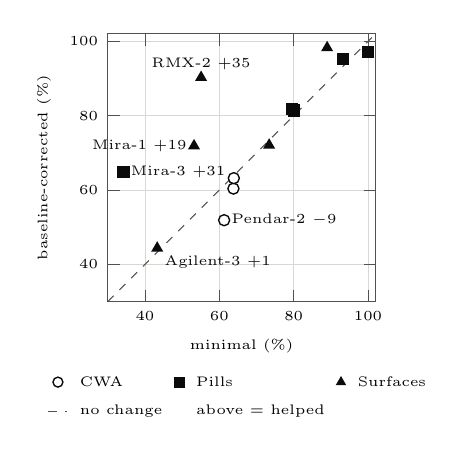
\begin{tikzpicture}
\begin{axis}[width=3.4cm,height=3.4cm,scale only axis,xmin=30,xmax=102,ymin=30,ymax=102,
  xtick={40,60,80,100},ytick={40,60,80,100},tick label style={font=\tiny},label style={font=\tiny},
  xlabel={minimal (\%)},ylabel={baseline-corrected (\%)},xmajorgrids,ymajorgrids,grid style={cGrid,very thin},
  axis line style={cInk2},tick style={cInk2},clip=false]
\addplot[cInk2,dashed,thin,domain=30:102] {x};
\addplot[only marks,mark=*,mark size=2.0pt,color=cInk,mark options={fill=white,draw=cInk,line width=0.5pt}] coordinates {(63.8,60.4) (61.3,51.9) (63.9,63.2)};
\addplot[only marks,mark=square*,mark size=2.0pt,color=cInk,mark options={fill=cInk,draw=cInk,line width=0.5pt}] coordinates {(80.1,81.4) (93.3,95.2) (34.2,64.8) (79.6,81.8) (100.0,97.1)};
\addplot[only marks,mark=triangle*,mark size=2.0pt,color=cInk,mark options={fill=cInk,draw=cInk,line width=0.5pt}] coordinates {(43.3,44.4) (53.2,71.9) (89.0,98.3) (73.4,72.1) (55.1,90.3)};
\node[font=\tiny,anchor=west,inner sep=2.5pt,text=cInk] at (axis cs:34.2,64.8) {Mira-3 +31};
\node[font=\tiny,anchor=south,inner sep=2.5pt,text=cInk] at (axis cs:55.1,90.3) {RMX-2 +35};
\node[font=\tiny,anchor=east,inner sep=2.5pt,text=cInk] at (axis cs:53.2,71.9) {Mira-1 +19};
\node[font=\tiny,anchor=west,inner sep=2.5pt,text=cInk] at (axis cs:61.3,51.9) {Pendar-2 $-$9};
\node[font=\tiny,anchor=north west,inner sep=2.5pt,text=cInk] at (axis cs:43.3,44.4) {Agilent-3 +1};
\end{axis}
\matrix[anchor=north,font=\tiny,column sep=1pt] at (1.7,-0.72) {\draw[fill=white,draw=cInk,line width=0.5pt] plot[mark=*,mark size=1.8pt] coordinates {(0,0)}; & \node[anchor=west]{CWA}; &\draw[fill=cInk,draw=cInk] plot[mark=square*,mark size=1.8pt] coordinates {(0,0)}; & \node[anchor=west]{Pills}; &\draw[fill=cInk,draw=cInk] plot[mark=triangle*,mark size=1.8pt] coordinates {(0,0)}; & \node[anchor=west]{Surfaces}; \\\draw[cInk2,dashed] (-0.12,0) -- (0.12,0); & \node[anchor=west]{no change}; & & \node[anchor=west]{above = helped}; & & \\};
\end{tikzpicture}

\column{0.35\textwidth}
\centering
\scriptsize\textbf{Per substrate, held-out instrument}\par\smallskip
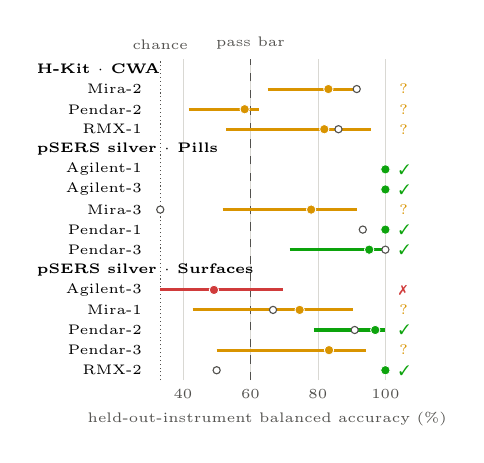
\begin{tikzpicture}[font=\tiny]
\draw[cGrid,very thin] (0.429,0) -- (0.429,4.080);
\node[anchor=north,text=cInk2] at (0.429,0) {40};
\draw[cGrid,very thin] (1.286,0) -- (1.286,4.080);
\node[anchor=north,text=cInk2] at (1.286,0) {60};
\draw[cGrid,very thin] (2.143,0) -- (2.143,4.080);
\node[anchor=north,text=cInk2] at (2.143,0) {80};
\draw[cGrid,very thin] (3.000,0) -- (3.000,4.080);
\node[anchor=north,text=cInk2] at (3.000,0) {100};
\draw[cInk2,dashed] (1.286,0) -- (1.286,4.080);
\draw[cInk2,densely dotted] (0.143,0) -- (0.143,4.080);
\node[anchor=south,text=cInk2,align=center,font=\tiny] at (1.286,4.080) {pass bar};
\node[anchor=south,text=cInk2,font=\tiny] at (0.141,4.080) {chance};
\node[anchor=west,font=\tiny\bfseries] at (-1.55,3.953) {H-Kit $\cdot$ CWA};
\node[anchor=east,inner sep=1pt] at (-0.05,3.698) {Mira-2};
\draw[sWarn,line width=1.1pt] (1.504,3.698) -- (2.683,3.698);
\draw[cInk2,fill=white,line width=0.4pt] (2.636,3.698) circle (1.3pt);
\fill[sWarn,draw=white,line width=0.3pt] (2.276,3.698) circle (1.7pt);
\node[anchor=west,text=sWarn] at (3.050,3.698) {?};
\node[anchor=east,inner sep=1pt] at (-0.05,3.442) {Pendar-2};
\draw[sWarn,line width=1.1pt] (0.501,3.442) -- (1.393,3.442);
\draw[cInk2,fill=white,line width=0.4pt] (1.213,3.442) circle (1.3pt);
\fill[sWarn,draw=white,line width=0.3pt] (1.213,3.442) circle (1.7pt);
\node[anchor=west,text=sWarn] at (3.050,3.442) {?};
\node[anchor=east,inner sep=1pt] at (-0.05,3.188) {RMX-1};
\draw[sWarn,line width=1.1pt] (0.977,3.188) -- (2.820,3.188);
\draw[cInk2,fill=white,line width=0.4pt] (2.404,3.188) circle (1.3pt);
\fill[sWarn,draw=white,line width=0.3pt] (2.224,3.188) circle (1.7pt);
\node[anchor=west,text=sWarn] at (3.050,3.188) {?};
\node[anchor=west,font=\tiny\bfseries] at (-1.55,2.933) {pSERS silver $\cdot$ Pills};
\node[anchor=east,inner sep=1pt] at (-0.05,2.678) {Agilent-1};
\draw[sGood,line width=1.1pt] (3.000,2.678) -- (3.000,2.678);
\draw[cInk2,fill=white,line width=0.4pt] (3.000,2.678) circle (1.3pt);
\fill[sGood,draw=white,line width=0.3pt] (3.000,2.678) circle (1.7pt);
\node[anchor=west,text=sGood] at (3.050,2.678) {\ding{51}};
\node[anchor=east,inner sep=1pt] at (-0.05,2.423) {Agilent-3};
\draw[sGood,line width=1.1pt] (3.000,2.423) -- (3.000,2.423);
\draw[cInk2,fill=white,line width=0.4pt] (3.000,2.423) circle (1.3pt);
\fill[sGood,draw=white,line width=0.3pt] (3.000,2.423) circle (1.7pt);
\node[anchor=west,text=sGood] at (3.050,2.423) {\ding{51}};
\node[anchor=east,inner sep=1pt] at (-0.05,2.167) {Mira-3};
\draw[sWarn,line width=1.1pt] (0.934,2.167) -- (2.644,2.167);
\draw[cInk2,fill=white,line width=0.4pt] (0.141,2.167) circle (1.3pt);
\fill[sWarn,draw=white,line width=0.3pt] (2.057,2.167) circle (1.7pt);
\node[anchor=west,text=sWarn] at (3.050,2.167) {?};
\node[anchor=east,inner sep=1pt] at (-0.05,1.913) {Pendar-1};
\draw[sGood,line width=1.1pt] (3.000,1.913) -- (3.000,1.913);
\draw[cInk2,fill=white,line width=0.4pt] (2.713,1.913) circle (1.3pt);
\fill[sGood,draw=white,line width=0.3pt] (3.000,1.913) circle (1.7pt);
\node[anchor=west,text=sGood] at (3.050,1.913) {\ding{51}};
\node[anchor=east,inner sep=1pt] at (-0.05,1.658) {Pendar-3};
\draw[sGood,line width=1.1pt] (1.783,1.658) -- (3.000,1.658);
\draw[cInk2,fill=white,line width=0.4pt] (3.000,1.658) circle (1.3pt);
\fill[sGood,draw=white,line width=0.3pt] (2.794,1.658) circle (1.7pt);
\node[anchor=west,text=sGood] at (3.050,1.658) {\ding{51}};
\node[anchor=west,font=\tiny\bfseries] at (-1.55,1.402) {pSERS silver $\cdot$ Surfaces};
\node[anchor=east,inner sep=1pt] at (-0.05,1.147) {Agilent-3};
\draw[sCrit,line width=1.1pt] (0.141,1.147) -- (1.706,1.147);
\draw[cInk2,fill=white,line width=0.4pt] (0.823,1.147) circle (1.3pt);
\fill[sCrit,draw=white,line width=0.3pt] (0.823,1.147) circle (1.7pt);
\node[anchor=west,text=sCrit] at (3.050,1.147) {\ding{55}};
\node[anchor=east,inner sep=1pt] at (-0.05,0.893) {Mira-1};
\draw[sWarn,line width=1.1pt] (0.553,0.893) -- (2.593,0.893);
\draw[cInk2,fill=white,line width=0.4pt] (1.573,0.893) circle (1.3pt);
\fill[sWarn,draw=white,line width=0.3pt] (1.911,0.893) circle (1.7pt);
\node[anchor=west,text=sWarn] at (3.050,0.893) {?};
\node[anchor=east,inner sep=1pt] at (-0.05,0.638) {Pendar-2};
\draw[sGood,line width=1.1pt] (2.091,0.638) -- (3.000,0.638);
\draw[cInk2,fill=white,line width=0.4pt] (2.610,0.638) circle (1.3pt);
\fill[sGood,draw=white,line width=0.3pt] (2.871,0.638) circle (1.7pt);
\node[anchor=west,text=sGood] at (3.050,0.638) {\ding{51}};
\node[anchor=east,inner sep=1pt] at (-0.05,0.382) {Pendar-3};
\draw[sWarn,line width=1.1pt] (0.857,0.382) -- (2.760,0.382);
\draw[cInk2,fill=white,line width=0.4pt] (2.284,0.382) circle (1.3pt);
\fill[sWarn,draw=white,line width=0.3pt] (2.284,0.382) circle (1.7pt);
\node[anchor=west,text=sWarn] at (3.050,0.382) {?};
\node[anchor=east,inner sep=1pt] at (-0.05,0.127) {RMX-2};
\draw[sGood,line width=1.1pt] (3.000,0.127) -- (3.000,0.127);
\draw[cInk2,fill=white,line width=0.4pt] (0.857,0.127) circle (1.3pt);
\fill[sGood,draw=white,line width=0.3pt] (3.000,0.127) circle (1.7pt);
\node[anchor=west,text=sGood] at (3.050,0.127) {\ding{51}};
\node[anchor=north,text=cInk2] at (1.500,-0.28) {held-out-instrument balanced accuracy (\%)};
\end{tikzpicture}

\end{columns}
\takeaway{Correction rescues background-heavy instruments (Mira-3 +31, RMX-2 +35 points) but lowers every CWA instrument (by 1--9 points). pSERS silver passes 6 of 10 instrument tests. The field log recorded detection for 75\% of pSERS and 23\% of H-Kit measurements.}
\src{Substrate panel (Extra Trees, chosen after the results): dot and bar = corrected estimate and 95\% interval; open circle = minimal. Pass: lower bound $\geq$60\% and $\leq$10-point loss. The pre-planned test found no substrate passed; NRC and GaN/polymer had too few samples.}
\end{frame}

% -------------------------------------------------------------------------- 9
\begin{frame}{Paper 1: what this dataset supports now}
\textbf{Working title:} Chemical identification on unseen handheld Raman instruments: a leakage-controlled benchmark on a multi-instrument SERS field trial

\begin{columns}[T,onlytextwidth]
\column{0.50\textwidth}
\textbf{Contributions}
\begin{itemize}\small
  \item Curated field-trial dataset with its coverage matrix.
  \item Strict test: unseen instrument \emph{and} unseen samples.
  \item Tree models and compact CNNs perform alike.
  \item Baseline correction: +5 to +7 points, but instrument-dependent.
  \item Substrate performance across instruments is condition-specific.
\end{itemize}

\smallskip
{\small\textbf{Candidate journals}}\par
\scriptsize Analyst (first choice) \,$\cdot$\, Analytical Chemistry (reach) \,$\cdot$\, Applied Spectroscopy \,$\cdot$\, Analytica Chimica Acta \,$\cdot$\, J.\ Raman Spectrosc.; Scientific Data if the data can be released
\column{0.48\textwidth}
\textbf{Closest prior work}\par
\scriptsize
\begin{itemize}
  \item Fornasaro et al.\ and Guo et al., \emph{Anal.\ Chem.} 2020: spectra differ across labs and devices --- variability measured, identification not benchmarked.
  \item Mahmud et al., \emph{Spectrochim.\ Acta A} 2026: maps 4 portable SERS instruments to a lab instrument --- bacteria, one substrate.
  \item Lai et al., \emph{Anal.\ Chem.} 2025; She et al., \emph{Anal.\ Chem.} 2026: transfer models between devices --- need data from the new instrument.
  \item Mirsafavi et al., \emph{Analyst} 2020; Wilson et al., \emph{Sens.\ Actuators B} 2021: SERS of fentanyl and 4-ANPP --- one instrument.
\end{itemize}
\textbf{Gap:} no study tests an unseen handheld instrument with sample-grouped splits across several substrates and vendors.

\end{columns}
\src{The contribution is the test protocol and a rare dataset, not a new method. Classical $\approx$ CNN agrees with recent Raman benchmarks (Sineesh \& Kamsali, \emph{Digital Discovery} 2026). Checked 20 October 2026 against Crossref; full list in backup.}
\end{frame}

% -------------------------------------------------------------------------- 10
\begin{frame}{What a proper dataset needs}
\begin{columns}[T,onlytextwidth]
\column{0.40\textwidth}
\centering
\scriptsize\textbf{Independent samples per chemical $\times$ substrate}\par\smallskip
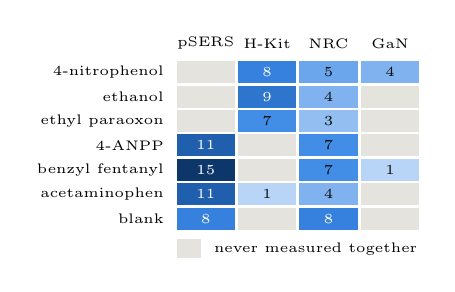
\begin{tikzpicture}[x=0.78cm,y=0.31cm,font=\tiny]
\fill[cNA] (0,6) rectangle +(0.95,0.9);
\fill[fill={rgb,255:red,53;green,129;blue,221}] (1,6) rectangle +(0.95,0.9);
\node[text=white] at (1.475,6.45) {8};
\fill[fill={rgb,255:red,107;green,166;blue,236}] (2,6) rectangle +(0.95,0.9);
\node[text=cInk] at (2.475,6.45) {5};
\fill[fill={rgb,255:red,127;green,178;blue,239}] (3,6) rectangle +(0.95,0.9);
\node[text=cInk] at (3.475,6.45) {4};
\fill[cNA] (0,5) rectangle +(0.95,0.9);
\fill[fill={rgb,255:red,45;green,117;blue,205}] (1,5) rectangle +(0.95,0.9);
\node[text=white] at (1.475,5.45) {9};
\fill[fill={rgb,255:red,127;green,178;blue,239}] (2,5) rectangle +(0.95,0.9);
\node[text=cInk] at (2.475,5.45) {4};
\fill[cNA] (3,5) rectangle +(0.95,0.9);
\fill[cNA] (0,4) rectangle +(0.95,0.9);
\fill[fill={rgb,255:red,66;green,141;blue,230}] (1,4) rectangle +(0.95,0.9);
\node[text=cInk] at (1.475,4.45) {7};
\fill[fill={rgb,255:red,146;green,190;blue,242}] (2,4) rectangle +(0.95,0.9);
\node[text=cInk] at (2.475,4.45) {3};
\fill[cNA] (3,4) rectangle +(0.95,0.9);
\fill[fill={rgb,255:red,32;green,95;blue,174}] (0,3) rectangle +(0.95,0.9);
\node[text=white] at (0.475,3.45) {11};
\fill[cNA] (1,3) rectangle +(0.95,0.9);
\fill[fill={rgb,255:red,66;green,141;blue,230}] (2,3) rectangle +(0.95,0.9);
\node[text=cInk] at (2.475,3.45) {7};
\fill[cNA] (3,3) rectangle +(0.95,0.9);
\fill[fill={rgb,255:red,13;green,54;blue,107}] (0,2) rectangle +(0.95,0.9);
\node[text=white] at (0.475,2.45) {15};
\fill[cNA] (1,2) rectangle +(0.95,0.9);
\fill[fill={rgb,255:red,66;green,141;blue,230}] (2,2) rectangle +(0.95,0.9);
\node[text=cInk] at (2.475,2.45) {7};
\fill[fill={rgb,255:red,184;green,213;blue,248}] (3,2) rectangle +(0.95,0.9);
\node[text=cInk] at (3.475,2.45) {1};
\fill[fill={rgb,255:red,32;green,95;blue,174}] (0,1) rectangle +(0.95,0.9);
\node[text=white] at (0.475,1.45) {11};
\fill[fill={rgb,255:red,184;green,213;blue,248}] (1,1) rectangle +(0.95,0.9);
\node[text=cInk] at (1.475,1.45) {1};
\fill[fill={rgb,255:red,127;green,178;blue,239}] (2,1) rectangle +(0.95,0.9);
\node[text=cInk] at (2.475,1.45) {4};
\fill[cNA] (3,1) rectangle +(0.95,0.9);
\fill[fill={rgb,255:red,53;green,129;blue,221}] (0,0) rectangle +(0.95,0.9);
\node[text=white] at (0.475,0.45) {8};
\fill[cNA] (1,0) rectangle +(0.95,0.9);
\fill[fill={rgb,255:red,53;green,129;blue,221}] (2,0) rectangle +(0.95,0.9);
\node[text=white] at (2.475,0.45) {8};
\fill[cNA] (3,0) rectangle +(0.95,0.9);
\node[anchor=south] at (0.475,7.0) {pSERS};
\node[anchor=south] at (1.475,7.0) {H-Kit};
\node[anchor=south] at (2.475,7.0) {NRC};
\node[anchor=south] at (3.475,7.0) {GaN};
\node[anchor=east] at (-0.05,6.45) {4-nitrophenol};
\node[anchor=east] at (-0.05,5.45) {ethanol};
\node[anchor=east] at (-0.05,4.45) {ethyl paraoxon};
\node[anchor=east] at (-0.05,3.45) {4-ANPP};
\node[anchor=east] at (-0.05,2.45) {benzyl fentanyl};
\node[anchor=east] at (-0.05,1.45) {acetaminophen};
\node[anchor=east] at (-0.05,0.45) {blank};
\fill[cNA] (0,-1.15) rectangle +(0.4,0.75); \node[anchor=west] at (0.45,-0.78) {never measured together};
\end{tikzpicture}

\par\medskip
\scriptsize\textbf{Why sample count matters (schematic)}\par\smallskip
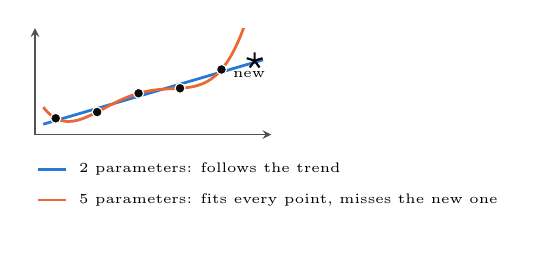
\begin{tikzpicture}
\begin{axis}[width=3.0cm,height=1.35cm,scale only axis,xmin=0.5,xmax=6.2,ymin=0,ymax=8.5,ticks=none,
  axis lines=left,axis line style={cInk2},clip=true]
\addplot[cBlue,line width=1pt] coordinates {(0.700,0.829) (0.745,0.872) (0.789,0.915) (0.834,0.959) (0.878,1.002) (0.923,1.045) (0.967,1.088) (1.012,1.131) (1.056,1.175) (1.101,1.218) (1.145,1.261) (1.190,1.304) (1.234,1.347) (1.279,1.391) (1.324,1.434) (1.368,1.477) (1.413,1.520) (1.457,1.563) (1.502,1.607) (1.546,1.650) (1.591,1.693) (1.635,1.736) (1.680,1.779) (1.724,1.823) (1.769,1.866) (1.813,1.909) (1.858,1.952) (1.903,1.995) (1.947,2.039) (1.992,2.082) (2.036,2.125) (2.081,2.168) (2.125,2.211) (2.170,2.255) (2.214,2.298) (2.259,2.341) (2.303,2.384) (2.348,2.427) (2.392,2.471) (2.437,2.514) (2.482,2.557) (2.526,2.600) (2.571,2.643) (2.615,2.687) (2.660,2.730) (2.704,2.773) (2.749,2.816) (2.793,2.859) (2.838,2.903) (2.882,2.946) (2.927,2.989) (2.971,3.032) (3.016,3.075) (3.061,3.119) (3.105,3.162) (3.150,3.205) (3.194,3.248) (3.239,3.291) (3.283,3.335) (3.328,3.378) (3.372,3.421) (3.417,3.464) (3.461,3.508) (3.506,3.551) (3.550,3.594) (3.595,3.637) (3.639,3.680) (3.684,3.724) (3.729,3.767) (3.773,3.810) (3.818,3.853) (3.862,3.896) (3.907,3.940) (3.951,3.983) (3.996,4.026) (4.040,4.069) (4.085,4.112) (4.129,4.156) (4.174,4.199) (4.218,4.242) (4.263,4.285) (4.308,4.328) (4.352,4.372) (4.397,4.415) (4.441,4.458) (4.486,4.501) (4.530,4.544) (4.575,4.588) (4.619,4.631) (4.664,4.674) (4.708,4.717) (4.753,4.760) (4.797,4.804) (4.842,4.847) (4.887,4.890) (4.931,4.933) (4.976,4.976) (5.020,5.020) (5.065,5.063) (5.109,5.106) (5.154,5.149) (5.198,5.192) (5.243,5.236) (5.287,5.279) (5.332,5.322) (5.376,5.365) (5.421,5.408) (5.466,5.452) (5.510,5.495) (5.555,5.538) (5.599,5.581) (5.644,5.624) (5.688,5.668) (5.733,5.711) (5.777,5.754) (5.822,5.797) (5.866,5.840) (5.911,5.884) (5.955,5.927) (6.000,5.970)};
\addplot[cOrange,line width=1pt] coordinates {(0.700,2.189) (0.745,2.008) (0.789,1.845) (0.834,1.700) (0.878,1.571) (0.923,1.459) (0.967,1.362) (1.012,1.280) (1.056,1.211) (1.101,1.155) (1.145,1.112) (1.190,1.080) (1.234,1.060) (1.279,1.049) (1.324,1.048) (1.368,1.056) (1.413,1.072) (1.457,1.096) (1.502,1.127) (1.546,1.165) (1.591,1.208) (1.635,1.257) (1.680,1.311) (1.724,1.369) (1.769,1.432) (1.813,1.497) (1.858,1.566) (1.903,1.637) (1.947,1.711) (1.992,1.786) (2.036,1.862) (2.081,1.940) (2.125,2.018) (2.170,2.096) (2.214,2.174) (2.259,2.252) (2.303,2.330) (2.348,2.406) (2.392,2.481) (2.437,2.555) (2.482,2.628) (2.526,2.698) (2.571,2.767) (2.615,2.833) (2.660,2.897) (2.704,2.959) (2.749,3.018) (2.793,3.074) (2.838,3.128) (2.882,3.179) (2.927,3.227) (2.971,3.272) (3.016,3.315) (3.061,3.354) (3.105,3.391) (3.150,3.425) (3.194,3.456) (3.239,3.484) (3.283,3.510) (3.328,3.533) (3.372,3.553) (3.417,3.572) (3.461,3.588) (3.506,3.603) (3.550,3.615) (3.595,3.626) (3.639,3.636) (3.684,3.645) (3.729,3.653) (3.773,3.660) (3.818,3.667) (3.862,3.674) (3.907,3.682) (3.951,3.690) (3.996,3.699) (4.040,3.710) (4.085,3.722) (4.129,3.737) (4.174,3.754) (4.218,3.775) (4.263,3.799) (4.308,3.827) (4.352,3.860) (4.397,3.897) (4.441,3.940) (4.486,3.990) (4.530,4.046) (4.575,4.109) (4.619,4.180) (4.664,4.260) (4.708,4.348) (4.753,4.447) (4.797,4.555) (4.842,4.675) (4.887,4.807) (4.931,4.951) (4.976,5.108) (5.020,5.279) (5.065,5.465) (5.109,5.667) (5.154,5.884) (5.198,6.119) (5.243,6.372) (5.287,6.643) (5.332,6.935) (5.376,7.246) (5.421,7.579) (5.466,7.935) (5.510,8.314) (5.555,8.717) (5.599,9.000) (5.644,9.000) (5.688,9.000) (5.733,9.000) (5.777,9.000) (5.822,9.000) (5.866,9.000) (5.911,9.000) (5.955,9.000) (6.000,9.000)};
\addplot[only marks,mark=*,mark size=1.8pt,color=cInk,mark options={fill=cInk,draw=white}] coordinates {(1.0,1.3) (2.0,1.8) (3.0,3.3) (4.0,3.7) (5.0,5.2)};
\addplot[only marks,mark=star,mark size=3pt,color=cInk,line width=0.8pt] coordinates {(5.8,5.9)};
\node[font=\tiny,anchor=north west,inner sep=1pt] at (axis cs:5.2,5.300000000000001) {new};
\end{axis}
\matrix[anchor=north west,font=\tiny,row sep=0pt,column sep=1pt] at (-0.1,-0.12) {\draw[cBlue,line width=1pt] (0,0) -- (0.35,0); & \node[anchor=west]{2 parameters: follows the trend}; \\\draw[cOrange,line width=1pt] (0,0) -- (0.35,0); & \node[anchor=west]{5 parameters: fits every point, misses the new one}; \\};
\end{tikzpicture}

\column{0.58\textwidth}
\small
\textbf{1. Fill the matrix.} A model separates two effects only if they vary independently. Here H-Kit met only CWA chemicals and pSERS only Pills/Surfaces chemicals. Needed: every chemical on every substrate and instrument, several independent samples per cell.

\medskip
\textbf{2. Ground truth for each effect:} pure-analyte Raman references, substrate-only blanks, instrument calibration standards; otherwise a model's ``chemical part'' cannot be checked.

\medskip
\textbf{3. Enough independent samples.} Our CNN has 208,691 adjustable parameters for 69 samples ($\approx$3,000 per sample). Extra parameters let a model fit the training data exactly yet miss new samples (left, bottom).

\medskip
\colorbox{cTake}{\parbox{\dimexpr\linewidth-2\fboxsep\relax}{\textbf{Illustrative design:} (6 analytes $\times$ 3 concentrations + 1 blank) $\times$ 4 substrates $\times$ 5 preparations = 380 independent samples (5.5$\times$ today), each read on 4 instruments, including $\geq$3 units of one brand.}}
\end{columns}
\src{Theory agrees: without labelled factors, disentanglement cannot be learned (Locatello et al., ICML 2019); correlated factors stay entangled (Tr\"auble et al., ICML 2021). Schematic uses five invented points; no exact ``samples $>$ parameters'' rule exists.}
\end{frame}

% -------------------------------------------------------------------------- 11
\begin{frame}{Paper 2: the original VAE goal, with a designed dataset}
\textbf{Working title:} Separating analyte, substrate and instrument contributions in SERS spectra with structured variational autoencoders

\begin{columns}[T,onlytextwidth]
\column{0.50\textwidth}
\textbf{How it would be tested}
\begin{itemize}\small
  \item Recover each analyte's reference spectrum from its SERS spectra.
  \item Predict chemical $\times$ substrate $\times$ instrument combinations deliberately left out of training.
  \item Compare against the Paper~1 benchmark methods.
\end{itemize}
\textbf{Why Paper 1 comes first}\par\small
Paper 1 shows the instrument effect dominates, and why separating it requires a crossed design.

\medskip
\textbf{Candidate journals}\par
\scriptsize Analytical Chemistry (ACS) \,$\cdot$\, Digital Discovery (RSC) \,$\cdot$\, Machine Learning: Science and Technology (IOP) \,$\cdot$\, Nature Communications (stretch) \,$\cdot$\, plus a Scientific Data descriptor for the dataset
\column{0.48\textwidth}
\textbf{Closest prior work}\par
\scriptsize
\begin{itemize}
  \item Fornasaro et al., \emph{Anal.\ Chem.} 2020: 15 labs, 6 SERS methods --- but one analyte; authors caution against extrapolating to other substrates.
  \item Mahmud et al., \emph{Spectrochim.\ Acta A} 2026: 20 analytes, 5 instruments --- but one substrate.
  \item Abram \& McCloskey, \emph{Biomolecules} 2023: a VAE separates instrument type --- in mass spectrometry.
  \item Lotfollahi et al., \emph{Mol.\ Syst.\ Biol.} 2023: predicts unseen drug $\times$ cell-type combinations --- a template from biology.
\end{itemize}
\textbf{Gap:} no crossed analyte $\times$ substrate $\times$ instrument SERS dataset with disentangled models was found.

\end{columns}
\src{Literature checked 20 October 2026 against Crossref and publisher/proceedings pages; repeat in Scopus before submission. Full list in backup.}
\end{frame}

% -------------------------------------------------------------------------- 12
\begin{frame}[t]{For discussion}\vspace{0.6em}
\begin{enumerate}
  \item \textbf{Publication.} Can results from the NATO trial data be published? Who must approve, who are co-authors, and is there a citable trial report (NATO SET-292, Aberdeen, March 2024)?
  \item \textbf{Route.} Paper 1 now with this dataset; Paper 2 requires new measurements.
  \item \textbf{New data.} Which analytes, substrates and instruments could NRC measure? Are $\geq$3 units of one brand available? Can one SERS chip be read on several instruments before it degrades?
  \item \textbf{Chemistry.} Why might the Mira units fail without baseline correction (Mira-1 also failed its system check)? Was ethyl paraoxon deposited from an ethanol solution?
  \item \textbf{Next experiments.} 1--2-sample calibration on a new instrument; robustness to added noise and background; other normalizations. Which matter most for the paper?
\end{enumerate}
\end{frame}

% ========================================================================== appendix
\appendix

\begin{frame}{Backup: how the test was kept fair}
\centering
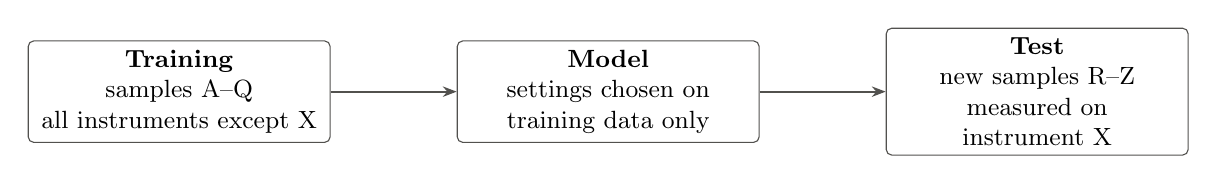
\begin{tikzpicture}[font=\small,
  box/.style={draw=cInk2,rounded corners=2pt,align=center,minimum height=1.1cm,text width=3.6cm,fill=white},
  arr/.style={-{Stealth[length=5pt]},cInk2,line width=0.8pt}]
\node[box] (train) {\textbf{Training}\\samples A--Q\\all instruments except X};
\node[box,right=1.6cm of train] (model) {\textbf{Model}\\settings chosen on\\training data only};
\node[box,right=1.6cm of model] (test) {\textbf{Test}\\new samples R--Z\\measured on instrument X};
\draw[arr] (train) -- (model);
\draw[arr] (model) -- (test);
\end{tikzpicture}

\vspace{0.8em}
\begin{itemize}\small
  \item Every spectrum of one physical sample stays on one side of the split (four folds, repeated five times).
  \item The held-out instrument contributes nothing to training, preprocessing statistics, model selection, calibration or stopping.
  \item 13 station--instrument combinations have enough samples for this test (CWA: 3, Pills: 5, Surfaces: 5).
  \item Scores use the same method as the 14 September report, so the 68.5\% Extra Trees figure is unchanged.
\end{itemize}
\end{frame}

\begin{frame}{Backup: all confusion matrices, baseline-corrected}
\centering
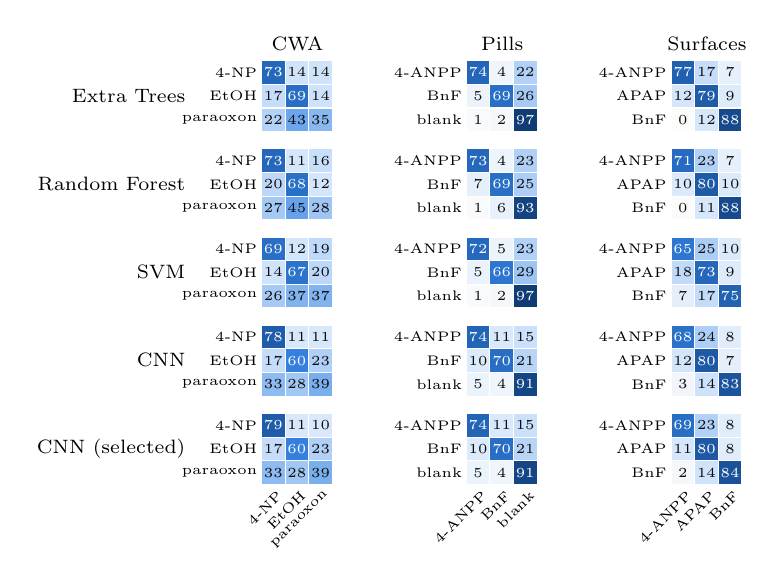
\begin{tikzpicture}[font=\tiny]
\fill[fill={rgb,255:red,36;green,104;blue,188}] (1.600,5.080) rectangle +(0.285,0.285);
\node[text=white] at (1.743,5.223) {73};
\fill[fill={rgb,255:red,207;green,227;blue,251}] (1.900,5.080) rectangle +(0.285,0.285);
\node[text=cInk] at (2.042,5.223) {14};
\fill[fill={rgb,255:red,207;green,227;blue,251}] (2.200,5.080) rectangle +(0.285,0.285);
\node[text=cInk] at (2.343,5.223) {14};
\fill[fill={rgb,255:red,197;green,221;blue,250}] (1.600,4.780) rectangle +(0.285,0.285);
\node[text=cInk] at (1.743,4.923) {17};
\fill[fill={rgb,255:red,40;green,110;blue,196}] (1.900,4.780) rectangle +(0.285,0.285);
\node[text=white] at (2.042,4.923) {69};
\fill[fill={rgb,255:red,206;green,227;blue,251}] (2.200,4.780) rectangle +(0.285,0.285);
\node[text=cInk] at (2.343,4.923) {14};
\fill[fill={rgb,255:red,179;green,210;blue,247}] (1.600,4.480) rectangle +(0.285,0.285);
\node[text=cInk] at (1.743,4.623) {22};
\fill[fill={rgb,255:red,108;green,166;blue,236}] (1.900,4.480) rectangle +(0.285,0.285);
\node[text=cInk] at (2.042,4.623) {43};
\fill[fill={rgb,255:red,137;green,184;blue,241}] (2.200,4.480) rectangle +(0.285,0.285);
\node[text=cInk] at (2.343,4.623) {35};
\node[anchor=east,inner sep=1pt] at (1.580,5.223) {4-NP};
\node[anchor=east,inner sep=1pt] at (1.580,4.923) {EtOH};
\node[anchor=east,inner sep=1pt] at (1.580,4.623) {paraoxon};
\node[anchor=south,font=\scriptsize] at (2.050,5.380) {CWA};
\fill[fill={rgb,255:red,35;green,101;blue,184}] (4.200,5.080) rectangle +(0.285,0.285);
\node[text=white] at (4.343,5.223) {74};
\fill[fill={rgb,255:red,240;green,245;blue,251}] (4.500,5.080) rectangle +(0.285,0.285);
\node[text=cInk] at (4.643,5.223) {4};
\fill[fill={rgb,255:red,178;green,209;blue,247}] (4.800,5.080) rectangle +(0.285,0.285);
\node[text=cInk] at (4.942,5.223) {22};
\fill[fill={rgb,255:red,236;green,243;blue,251}] (4.200,4.780) rectangle +(0.285,0.285);
\node[text=cInk] at (4.343,4.923) {5};
\fill[fill={rgb,255:red,41;green,111;blue,198}] (4.500,4.780) rectangle +(0.285,0.285);
\node[text=white] at (4.643,4.923) {69};
\fill[fill={rgb,255:red,166;green,202;blue,245}] (4.800,4.780) rectangle +(0.285,0.285);
\node[text=cInk] at (4.942,4.923) {26};
\fill[fill={rgb,255:red,248;green,250;blue,251}] (4.200,4.480) rectangle +(0.285,0.285);
\node[text=cInk] at (4.343,4.623) {1};
\fill[fill={rgb,255:red,245;green,248;blue,251}] (4.500,4.480) rectangle +(0.285,0.285);
\node[text=cInk] at (4.643,4.623) {2};
\fill[fill={rgb,255:red,16;green,60;blue,117}] (4.800,4.480) rectangle +(0.285,0.285);
\node[text=white] at (4.942,4.623) {97};
\node[anchor=east,inner sep=1pt] at (4.180,5.223) {4-ANPP};
\node[anchor=east,inner sep=1pt] at (4.180,4.923) {BnF};
\node[anchor=east,inner sep=1pt] at (4.180,4.623) {blank};
\node[anchor=south,font=\scriptsize] at (4.650,5.380) {Pills};
\fill[fill={rgb,255:red,32;green,96;blue,176}] (6.800,5.080) rectangle +(0.285,0.285);
\node[text=white] at (6.943,5.223) {77};
\fill[fill={rgb,255:red,197;green,221;blue,250}] (7.100,5.080) rectangle +(0.285,0.285);
\node[text=cInk] at (7.243,5.223) {17};
\fill[fill={rgb,255:red,230;green,240;blue,251}] (7.400,5.080) rectangle +(0.285,0.285);
\node[text=cInk] at (7.543,5.223) {7};
\fill[fill={rgb,255:red,213;green,230;blue,251}] (6.800,4.780) rectangle +(0.285,0.285);
\node[text=cInk] at (6.943,4.923) {12};
\fill[fill={rgb,255:red,30;green,92;blue,170}] (7.100,4.780) rectangle +(0.285,0.285);
\node[text=white] at (7.243,4.923) {79};
\fill[fill={rgb,255:red,221;green,235;blue,251}] (7.400,4.780) rectangle +(0.285,0.285);
\node[text=cInk] at (7.543,4.923) {9};
\fill[fill={rgb,255:red,252;green,252;blue,251}] (6.800,4.480) rectangle +(0.285,0.285);
\node[text=cInk] at (6.943,4.623) {0};
\fill[fill={rgb,255:red,214;green,231;blue,251}] (7.100,4.480) rectangle +(0.285,0.285);
\node[text=cInk] at (7.243,4.623) {12};
\fill[fill={rgb,255:red,22;green,74;blue,141}] (7.400,4.480) rectangle +(0.285,0.285);
\node[text=white] at (7.543,4.623) {88};
\node[anchor=east,inner sep=1pt] at (6.780,5.223) {4-ANPP};
\node[anchor=east,inner sep=1pt] at (6.780,4.923) {APAP};
\node[anchor=east,inner sep=1pt] at (6.780,4.623) {BnF};
\node[anchor=south,font=\scriptsize] at (7.250,5.380) {Surfaces};
\node[anchor=east,font=\scriptsize] at (0.75,4.930) {Extra Trees};
\fill[fill={rgb,255:red,36;green,103;blue,187}] (1.600,3.960) rectangle +(0.285,0.285);
\node[text=white] at (1.743,4.103) {73};
\fill[fill={rgb,255:red,215;green,231;blue,251}] (1.900,3.960) rectangle +(0.285,0.285);
\node[text=cInk] at (2.042,4.103) {11};
\fill[fill={rgb,255:red,200;green,223;blue,250}] (2.200,3.960) rectangle +(0.285,0.285);
\node[text=cInk] at (2.343,4.103) {16};
\fill[fill={rgb,255:red,188;green,215;blue,248}] (1.600,3.660) rectangle +(0.285,0.285);
\node[text=cInk] at (1.743,3.803) {20};
\fill[fill={rgb,255:red,41;green,112;blue,199}] (1.900,3.660) rectangle +(0.285,0.285);
\node[text=white] at (2.042,3.803) {68};
\fill[fill={rgb,255:red,212;green,230;blue,251}] (2.200,3.660) rectangle +(0.285,0.285);
\node[text=cInk] at (2.343,3.803) {12};
\fill[fill={rgb,255:red,164;green,201;blue,245}] (1.600,3.360) rectangle +(0.285,0.285);
\node[text=cInk] at (1.743,3.503) {27};
\fill[fill={rgb,255:red,102;green,162;blue,235}] (1.900,3.360) rectangle +(0.285,0.285);
\node[text=cInk] at (2.042,3.503) {45};
\fill[fill={rgb,255:red,159;green,197;blue,244}] (2.200,3.360) rectangle +(0.285,0.285);
\node[text=cInk] at (2.343,3.503) {28};
\node[anchor=east,inner sep=1pt] at (1.580,4.103) {4-NP};
\node[anchor=east,inner sep=1pt] at (1.580,3.803) {EtOH};
\node[anchor=east,inner sep=1pt] at (1.580,3.503) {paraoxon};
\fill[fill={rgb,255:red,36;green,103;blue,187}] (4.200,3.960) rectangle +(0.285,0.285);
\node[text=white] at (4.343,4.103) {73};
\fill[fill={rgb,255:red,238;green,244;blue,251}] (4.500,3.960) rectangle +(0.285,0.285);
\node[text=cInk] at (4.643,4.103) {4};
\fill[fill={rgb,255:red,176;green,208;blue,247}] (4.800,3.960) rectangle +(0.285,0.285);
\node[text=cInk] at (4.942,4.103) {23};
\fill[fill={rgb,255:red,230;green,240;blue,251}] (4.200,3.660) rectangle +(0.285,0.285);
\node[text=cInk] at (4.343,3.803) {7};
\fill[fill={rgb,255:red,41;green,111;blue,198}] (4.500,3.660) rectangle +(0.285,0.285);
\node[text=white] at (4.643,3.803) {69};
\fill[fill={rgb,255:red,171;green,205;blue,246}] (4.800,3.660) rectangle +(0.285,0.285);
\node[text=cInk] at (4.942,3.803) {25};
\fill[fill={rgb,255:red,248;green,250;blue,251}] (4.200,3.360) rectangle +(0.285,0.285);
\node[text=cInk] at (4.343,3.503) {1};
\fill[fill={rgb,255:red,232;green,241;blue,251}] (4.500,3.360) rectangle +(0.285,0.285);
\node[text=cInk] at (4.643,3.503) {6};
\fill[fill={rgb,255:red,19;green,67;blue,128}] (4.800,3.360) rectangle +(0.285,0.285);
\node[text=white] at (4.942,3.503) {93};
\node[anchor=east,inner sep=1pt] at (4.180,4.103) {4-ANPP};
\node[anchor=east,inner sep=1pt] at (4.180,3.803) {BnF};
\node[anchor=east,inner sep=1pt] at (4.180,3.503) {blank};
\fill[fill={rgb,255:red,38;green,107;blue,193}] (6.800,3.960) rectangle +(0.285,0.285);
\node[text=white] at (6.943,4.103) {71};
\fill[fill={rgb,255:red,177;green,209;blue,247}] (7.100,3.960) rectangle +(0.285,0.285);
\node[text=cInk] at (7.243,4.103) {23};
\fill[fill={rgb,255:red,230;green,240;blue,251}] (7.400,3.960) rectangle +(0.285,0.285);
\node[text=cInk] at (7.543,4.103) {7};
\fill[fill={rgb,255:red,218;green,233;blue,251}] (6.800,3.660) rectangle +(0.285,0.285);
\node[text=cInk] at (6.943,3.803) {10};
\fill[fill={rgb,255:red,30;green,91;blue,167}] (7.100,3.660) rectangle +(0.285,0.285);
\node[text=white] at (7.243,3.803) {80};
\fill[fill={rgb,255:red,219;green,234;blue,251}] (7.400,3.660) rectangle +(0.285,0.285);
\node[text=cInk] at (7.543,3.803) {10};
\fill[fill={rgb,255:red,251;green,251;blue,251}] (6.800,3.360) rectangle +(0.285,0.285);
\node[text=cInk] at (6.943,3.503) {0};
\fill[fill={rgb,255:red,214;green,231;blue,251}] (7.100,3.360) rectangle +(0.285,0.285);
\node[text=cInk] at (7.243,3.503) {11};
\fill[fill={rgb,255:red,22;green,74;blue,141}] (7.400,3.360) rectangle +(0.285,0.285);
\node[text=white] at (7.543,3.503) {88};
\node[anchor=east,inner sep=1pt] at (6.780,4.103) {4-ANPP};
\node[anchor=east,inner sep=1pt] at (6.780,3.803) {APAP};
\node[anchor=east,inner sep=1pt] at (6.780,3.503) {BnF};
\node[anchor=east,font=\scriptsize] at (0.75,3.810) {Random Forest};
\fill[fill={rgb,255:red,40;green,111;blue,197}] (1.600,2.840) rectangle +(0.285,0.285);
\node[text=white] at (1.743,2.983) {69};
\fill[fill={rgb,255:red,212;green,230;blue,251}] (1.900,2.840) rectangle +(0.285,0.285);
\node[text=cInk] at (2.042,2.983) {12};
\fill[fill={rgb,255:red,190;green,217;blue,249}] (2.200,2.840) rectangle +(0.285,0.285);
\node[text=cInk] at (2.343,2.983) {19};
\fill[fill={rgb,255:red,207;green,227;blue,251}] (1.600,2.540) rectangle +(0.285,0.285);
\node[text=cInk] at (1.743,2.683) {14};
\fill[fill={rgb,255:red,43;green,115;blue,203}] (1.900,2.540) rectangle +(0.285,0.285);
\node[text=white] at (2.042,2.683) {67};
\fill[fill={rgb,255:red,188;green,215;blue,248}] (2.200,2.540) rectangle +(0.285,0.285);
\node[text=cInk] at (2.343,2.683) {20};
\fill[fill={rgb,255:red,166;green,202;blue,245}] (1.600,2.240) rectangle +(0.285,0.285);
\node[text=cInk] at (1.743,2.383) {26};
\fill[fill={rgb,255:red,129;green,180;blue,239}] (1.900,2.240) rectangle +(0.285,0.285);
\node[text=cInk] at (2.042,2.383) {37};
\fill[fill={rgb,255:red,129;green,180;blue,239}] (2.200,2.240) rectangle +(0.285,0.285);
\node[text=cInk] at (2.343,2.383) {37};
\node[anchor=east,inner sep=1pt] at (1.580,2.983) {4-NP};
\node[anchor=east,inner sep=1pt] at (1.580,2.683) {EtOH};
\node[anchor=east,inner sep=1pt] at (1.580,2.383) {paraoxon};
\fill[fill={rgb,255:red,36;green,105;blue,189}] (4.200,2.840) rectangle +(0.285,0.285);
\node[text=white] at (4.343,2.983) {72};
\fill[fill={rgb,255:red,236;green,243;blue,251}] (4.500,2.840) rectangle +(0.285,0.285);
\node[text=cInk] at (4.643,2.983) {5};
\fill[fill={rgb,255:red,177;green,209;blue,247}] (4.800,2.840) rectangle +(0.285,0.285);
\node[text=cInk] at (4.942,2.983) {23};
\fill[fill={rgb,255:red,234;green,242;blue,251}] (4.200,2.540) rectangle +(0.285,0.285);
\node[text=cInk] at (4.343,2.683) {5};
\fill[fill={rgb,255:red,45;green,117;blue,206}] (4.500,2.540) rectangle +(0.285,0.285);
\node[text=white] at (4.643,2.683) {66};
\fill[fill={rgb,255:red,157;green,197;blue,244}] (4.800,2.540) rectangle +(0.285,0.285);
\node[text=cInk] at (4.942,2.683) {29};
\fill[fill={rgb,255:red,248;green,250;blue,251}] (4.200,2.240) rectangle +(0.285,0.285);
\node[text=cInk] at (4.343,2.383) {1};
\fill[fill={rgb,255:red,245;green,248;blue,251}] (4.500,2.240) rectangle +(0.285,0.285);
\node[text=cInk] at (4.643,2.383) {2};
\fill[fill={rgb,255:red,15;green,60;blue,116}] (4.800,2.240) rectangle +(0.285,0.285);
\node[text=white] at (4.942,2.383) {97};
\node[anchor=east,inner sep=1pt] at (4.180,2.983) {4-ANPP};
\node[anchor=east,inner sep=1pt] at (4.180,2.683) {BnF};
\node[anchor=east,inner sep=1pt] at (4.180,2.383) {blank};
\fill[fill={rgb,255:red,46;green,118;blue,207}] (6.800,2.840) rectangle +(0.285,0.285);
\node[text=white] at (6.943,2.983) {65};
\fill[fill={rgb,255:red,171;green,205;blue,246}] (7.100,2.840) rectangle +(0.285,0.285);
\node[text=cInk] at (7.243,2.983) {25};
\fill[fill={rgb,255:red,219;green,234;blue,251}] (7.400,2.840) rectangle +(0.285,0.285);
\node[text=cInk] at (7.543,2.983) {10};
\fill[fill={rgb,255:red,193;green,218;blue,249}] (6.800,2.540) rectangle +(0.285,0.285);
\node[text=cInk] at (6.943,2.683) {18};
\fill[fill={rgb,255:red,36;green,103;blue,187}] (7.100,2.540) rectangle +(0.285,0.285);
\node[text=white] at (7.243,2.683) {73};
\fill[fill={rgb,255:red,222;green,235;blue,251}] (7.400,2.540) rectangle +(0.285,0.285);
\node[text=cInk] at (7.543,2.683) {9};
\fill[fill={rgb,255:red,228;green,239;blue,251}] (6.800,2.240) rectangle +(0.285,0.285);
\node[text=cInk] at (6.943,2.383) {7};
\fill[fill={rgb,255:red,196;green,220;blue,250}] (7.100,2.240) rectangle +(0.285,0.285);
\node[text=cInk] at (7.243,2.383) {17};
\fill[fill={rgb,255:red,33;green,98;blue,179}] (7.400,2.240) rectangle +(0.285,0.285);
\node[text=white] at (7.543,2.383) {75};
\node[anchor=east,inner sep=1pt] at (6.780,2.983) {4-ANPP};
\node[anchor=east,inner sep=1pt] at (6.780,2.683) {APAP};
\node[anchor=east,inner sep=1pt] at (6.780,2.383) {BnF};
\node[anchor=east,font=\scriptsize] at (0.75,2.690) {SVM};
\fill[fill={rgb,255:red,31;green,93;blue,171}] (1.600,1.720) rectangle +(0.285,0.285);
\node[text=white] at (1.743,1.863) {78};
\fill[fill={rgb,255:red,216;green,232;blue,251}] (1.900,1.720) rectangle +(0.285,0.285);
\node[text=cInk] at (2.042,1.863) {11};
\fill[fill={rgb,255:red,216;green,232;blue,251}] (2.200,1.720) rectangle +(0.285,0.285);
\node[text=cInk] at (2.343,1.863) {11};
\fill[fill={rgb,255:red,197;green,221;blue,250}] (1.600,1.420) rectangle +(0.285,0.285);
\node[text=cInk] at (1.743,1.563) {17};
\fill[fill={rgb,255:red,52;green,128;blue,220}] (1.900,1.420) rectangle +(0.285,0.285);
\node[text=white] at (2.042,1.563) {60};
\fill[fill={rgb,255:red,176;green,208;blue,247}] (2.200,1.420) rectangle +(0.285,0.285);
\node[text=cInk] at (2.343,1.563) {23};
\fill[fill={rgb,255:red,142;green,187;blue,241}] (1.600,1.120) rectangle +(0.285,0.285);
\node[text=cInk] at (1.743,1.263) {33};
\fill[fill={rgb,255:red,161;green,199;blue,244}] (1.900,1.120) rectangle +(0.285,0.285);
\node[text=cInk] at (2.042,1.263) {28};
\fill[fill={rgb,255:red,122;green,175;blue,238}] (2.200,1.120) rectangle +(0.285,0.285);
\node[text=cInk] at (2.343,1.263) {39};
\node[anchor=east,inner sep=1pt] at (1.580,1.863) {4-NP};
\node[anchor=east,inner sep=1pt] at (1.580,1.563) {EtOH};
\node[anchor=east,inner sep=1pt] at (1.580,1.263) {paraoxon};
\fill[fill={rgb,255:red,34;green,100;blue,182}] (4.200,1.720) rectangle +(0.285,0.285);
\node[text=white] at (4.343,1.863) {74};
\fill[fill={rgb,255:red,217;green,233;blue,251}] (4.500,1.720) rectangle +(0.285,0.285);
\node[text=cInk] at (4.643,1.863) {11};
\fill[fill={rgb,255:red,203;green,225;blue,251}] (4.800,1.720) rectangle +(0.285,0.285);
\node[text=cInk] at (4.942,1.863) {15};
\fill[fill={rgb,255:red,220;green,235;blue,251}] (4.200,1.420) rectangle +(0.285,0.285);
\node[text=cInk] at (4.343,1.563) {10};
\fill[fill={rgb,255:red,40;green,110;blue,196}] (4.500,1.420) rectangle +(0.285,0.285);
\node[text=white] at (4.643,1.563) {70};
\fill[fill={rgb,255:red,184;green,213;blue,248}] (4.800,1.420) rectangle +(0.285,0.285);
\node[text=cInk] at (4.942,1.563) {21};
\fill[fill={rgb,255:red,235;green,243;blue,251}] (4.200,1.120) rectangle +(0.285,0.285);
\node[text=cInk] at (4.343,1.263) {5};
\fill[fill={rgb,255:red,240;green,245;blue,251}] (4.500,1.120) rectangle +(0.285,0.285);
\node[text=cInk] at (4.643,1.263) {4};
\fill[fill={rgb,255:red,20;green,69;blue,133}] (4.800,1.120) rectangle +(0.285,0.285);
\node[text=white] at (4.942,1.263) {91};
\node[anchor=east,inner sep=1pt] at (4.180,1.863) {4-ANPP};
\node[anchor=east,inner sep=1pt] at (4.180,1.563) {BnF};
\node[anchor=east,inner sep=1pt] at (4.180,1.263) {blank};
\fill[fill={rgb,255:red,42;green,113;blue,200}] (6.800,1.720) rectangle +(0.285,0.285);
\node[text=white] at (6.943,1.863) {68};
\fill[fill={rgb,255:red,173;green,206;blue,246}] (7.100,1.720) rectangle +(0.285,0.285);
\node[text=cInk] at (7.243,1.863) {24};
\fill[fill={rgb,255:red,226;green,237;blue,251}] (7.400,1.720) rectangle +(0.285,0.285);
\node[text=cInk] at (7.543,1.863) {8};
\fill[fill={rgb,255:red,211;green,229;blue,251}] (6.800,1.420) rectangle +(0.285,0.285);
\node[text=cInk] at (6.943,1.563) {12};
\fill[fill={rgb,255:red,29;green,89;blue,165}] (7.100,1.420) rectangle +(0.285,0.285);
\node[text=white] at (7.243,1.563) {80};
\fill[fill={rgb,255:red,228;green,239;blue,251}] (7.400,1.420) rectangle +(0.285,0.285);
\node[text=cInk] at (7.543,1.563) {7};
\fill[fill={rgb,255:red,242;green,246;blue,251}] (6.800,1.120) rectangle +(0.285,0.285);
\node[text=cInk] at (6.943,1.263) {3};
\fill[fill={rgb,255:red,206;green,227;blue,251}] (7.100,1.120) rectangle +(0.285,0.285);
\node[text=cInk] at (7.243,1.263) {14};
\fill[fill={rgb,255:red,27;green,84;blue,157}] (7.400,1.120) rectangle +(0.285,0.285);
\node[text=white] at (7.543,1.263) {83};
\node[anchor=east,inner sep=1pt] at (6.780,1.863) {4-ANPP};
\node[anchor=east,inner sep=1pt] at (6.780,1.563) {APAP};
\node[anchor=east,inner sep=1pt] at (6.780,1.263) {BnF};
\node[anchor=east,font=\scriptsize] at (0.75,1.570) {CNN};
\fill[fill={rgb,255:red,30;green,92;blue,170}] (1.600,0.600) rectangle +(0.285,0.285);
\node[text=white] at (1.743,0.742) {79};
\fill[fill={rgb,255:red,216;green,232;blue,251}] (1.900,0.600) rectangle +(0.285,0.285);
\node[text=cInk] at (2.042,0.742) {11};
\fill[fill={rgb,255:red,217;green,233;blue,251}] (2.200,0.600) rectangle +(0.285,0.285);
\node[text=cInk] at (2.343,0.742) {10};
\fill[fill={rgb,255:red,197;green,221;blue,250}] (1.600,0.300) rectangle +(0.285,0.285);
\node[text=cInk] at (1.743,0.443) {17};
\fill[fill={rgb,255:red,52;green,128;blue,220}] (1.900,0.300) rectangle +(0.285,0.285);
\node[text=white] at (2.042,0.443) {60};
\fill[fill={rgb,255:red,176;green,208;blue,247}] (2.200,0.300) rectangle +(0.285,0.285);
\node[text=cInk] at (2.343,0.443) {23};
\fill[fill={rgb,255:red,142;green,187;blue,241}] (1.600,0.000) rectangle +(0.285,0.285);
\node[text=cInk] at (1.743,0.142) {33};
\fill[fill={rgb,255:red,161;green,199;blue,244}] (1.900,0.000) rectangle +(0.285,0.285);
\node[text=cInk] at (2.042,0.142) {28};
\fill[fill={rgb,255:red,122;green,175;blue,238}] (2.200,0.000) rectangle +(0.285,0.285);
\node[text=cInk] at (2.343,0.142) {39};
\node[anchor=east,inner sep=1pt] at (1.580,0.742) {4-NP};
\node[anchor=north east,rotate=45,inner sep=1pt] at (1.780,-0.020) {4-NP};
\node[anchor=east,inner sep=1pt] at (1.580,0.443) {EtOH};
\node[anchor=north east,rotate=45,inner sep=1pt] at (2.080,-0.020) {EtOH};
\node[anchor=east,inner sep=1pt] at (1.580,0.142) {paraoxon};
\node[anchor=north east,rotate=45,inner sep=1pt] at (2.380,-0.020) {paraoxon};
\fill[fill={rgb,255:red,34;green,100;blue,182}] (4.200,0.600) rectangle +(0.285,0.285);
\node[text=white] at (4.343,0.742) {74};
\fill[fill={rgb,255:red,217;green,233;blue,251}] (4.500,0.600) rectangle +(0.285,0.285);
\node[text=cInk] at (4.643,0.742) {11};
\fill[fill={rgb,255:red,203;green,225;blue,251}] (4.800,0.600) rectangle +(0.285,0.285);
\node[text=cInk] at (4.942,0.742) {15};
\fill[fill={rgb,255:red,220;green,235;blue,251}] (4.200,0.300) rectangle +(0.285,0.285);
\node[text=cInk] at (4.343,0.443) {10};
\fill[fill={rgb,255:red,40;green,110;blue,196}] (4.500,0.300) rectangle +(0.285,0.285);
\node[text=white] at (4.643,0.443) {70};
\fill[fill={rgb,255:red,184;green,213;blue,248}] (4.800,0.300) rectangle +(0.285,0.285);
\node[text=cInk] at (4.942,0.443) {21};
\fill[fill={rgb,255:red,235;green,243;blue,251}] (4.200,0.000) rectangle +(0.285,0.285);
\node[text=cInk] at (4.343,0.142) {5};
\fill[fill={rgb,255:red,240;green,245;blue,251}] (4.500,0.000) rectangle +(0.285,0.285);
\node[text=cInk] at (4.643,0.142) {4};
\fill[fill={rgb,255:red,20;green,69;blue,133}] (4.800,0.000) rectangle +(0.285,0.285);
\node[text=white] at (4.942,0.142) {91};
\node[anchor=east,inner sep=1pt] at (4.180,0.742) {4-ANPP};
\node[anchor=north east,rotate=45,inner sep=1pt] at (4.380,-0.020) {4-ANPP};
\node[anchor=east,inner sep=1pt] at (4.180,0.443) {BnF};
\node[anchor=north east,rotate=45,inner sep=1pt] at (4.680,-0.020) {BnF};
\node[anchor=east,inner sep=1pt] at (4.180,0.142) {blank};
\node[anchor=north east,rotate=45,inner sep=1pt] at (4.980,-0.020) {blank};
\fill[fill={rgb,255:red,40;green,110;blue,197}] (6.800,0.600) rectangle +(0.285,0.285);
\node[text=white] at (6.943,0.742) {69};
\fill[fill={rgb,255:red,177;green,209;blue,247}] (7.100,0.600) rectangle +(0.285,0.285);
\node[text=cInk] at (7.243,0.742) {23};
\fill[fill={rgb,255:red,226;green,237;blue,251}] (7.400,0.600) rectangle +(0.285,0.285);
\node[text=cInk] at (7.543,0.742) {8};
\fill[fill={rgb,255:red,214;green,231;blue,251}] (6.800,0.300) rectangle +(0.285,0.285);
\node[text=cInk] at (6.943,0.443) {11};
\fill[fill={rgb,255:red,29;green,89;blue,164}] (7.100,0.300) rectangle +(0.285,0.285);
\node[text=white] at (7.243,0.443) {80};
\fill[fill={rgb,255:red,225;green,237;blue,251}] (7.400,0.300) rectangle +(0.285,0.285);
\node[text=cInk] at (7.543,0.443) {8};
\fill[fill={rgb,255:red,244;green,248;blue,251}] (6.800,0.000) rectangle +(0.285,0.285);
\node[text=cInk] at (6.943,0.142) {2};
\fill[fill={rgb,255:red,207;green,227;blue,251}] (7.100,0.000) rectangle +(0.285,0.285);
\node[text=cInk] at (7.243,0.142) {14};
\fill[fill={rgb,255:red,26;green,82;blue,154}] (7.400,0.000) rectangle +(0.285,0.285);
\node[text=white] at (7.543,0.142) {84};
\node[anchor=east,inner sep=1pt] at (6.780,0.742) {4-ANPP};
\node[anchor=north east,rotate=45,inner sep=1pt] at (6.980,-0.020) {4-ANPP};
\node[anchor=east,inner sep=1pt] at (6.780,0.443) {APAP};
\node[anchor=north east,rotate=45,inner sep=1pt] at (7.280,-0.020) {APAP};
\node[anchor=east,inner sep=1pt] at (6.780,0.142) {BnF};
\node[anchor=north east,rotate=45,inner sep=1pt] at (7.580,-0.020) {BnF};
\node[anchor=east,font=\scriptsize] at (0.75,0.450) {CNN (selected)};
\end{tikzpicture}

\src{Rows = true chemical, columns = predicted; \% of each true chemical.}
\end{frame}

\begin{frame}{Backup: all confusion matrices, minimal preprocessing}
\centering
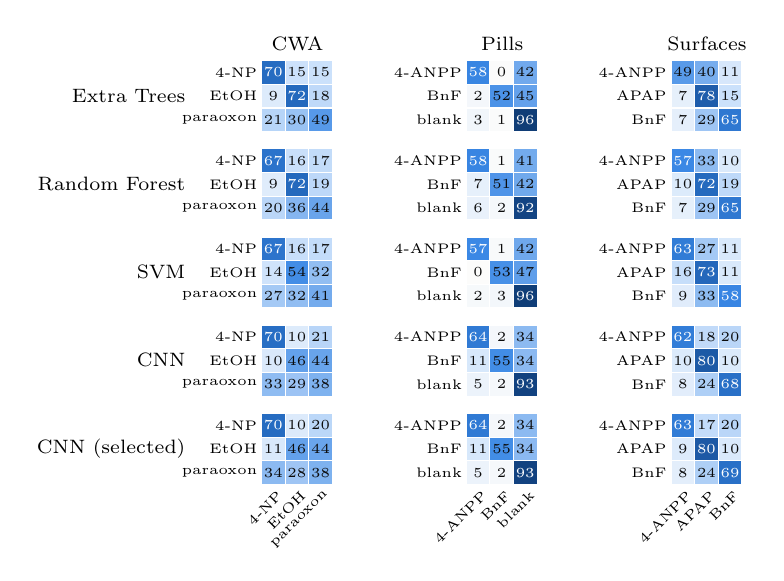
\begin{tikzpicture}[font=\tiny]
\fill[fill={rgb,255:red,38;green,108;blue,193}] (1.600,5.080) rectangle +(0.285,0.285);
\node[text=white] at (1.743,5.223) {70};
\fill[fill={rgb,255:red,204;green,225;blue,251}] (1.900,5.080) rectangle +(0.285,0.285);
\node[text=cInk] at (2.042,5.223) {15};
\fill[fill={rgb,255:red,203;green,225;blue,251}] (2.200,5.080) rectangle +(0.285,0.285);
\node[text=cInk] at (2.343,5.223) {15};
\fill[fill={rgb,255:red,221;green,235;blue,251}] (1.600,4.780) rectangle +(0.285,0.285);
\node[text=cInk] at (1.743,4.923) {9};
\fill[fill={rgb,255:red,36;green,105;blue,189}] (1.900,4.780) rectangle +(0.285,0.285);
\node[text=white] at (2.042,4.923) {72};
\fill[fill={rgb,255:red,191;green,217;blue,249}] (2.200,4.780) rectangle +(0.285,0.285);
\node[text=cInk] at (2.343,4.923) {18};
\fill[fill={rgb,255:red,183;green,213;blue,248}] (1.600,4.480) rectangle +(0.285,0.285);
\node[text=cInk] at (1.743,4.623) {21};
\fill[fill={rgb,255:red,152;green,194;blue,243}] (1.900,4.480) rectangle +(0.285,0.285);
\node[text=cInk] at (2.042,4.623) {30};
\fill[fill={rgb,255:red,87;green,153;blue,233}] (2.200,4.480) rectangle +(0.285,0.285);
\node[text=cInk] at (2.343,4.623) {49};
\node[anchor=east,inner sep=1pt] at (1.580,5.223) {4-NP};
\node[anchor=east,inner sep=1pt] at (1.580,4.923) {EtOH};
\node[anchor=east,inner sep=1pt] at (1.580,4.623) {paraoxon};
\node[anchor=south,font=\scriptsize] at (2.050,5.380) {CWA};
\fill[fill={rgb,255:red,56;green,133;blue,226}] (4.200,5.080) rectangle +(0.285,0.285);
\node[text=white] at (4.343,5.223) {58};
\fill[fill={rgb,255:red,251;green,251;blue,251}] (4.500,5.080) rectangle +(0.285,0.285);
\node[text=cInk] at (4.643,5.223) {0};
\fill[fill={rgb,255:red,113;green,169;blue,237}] (4.800,5.080) rectangle +(0.285,0.285);
\node[text=cInk] at (4.942,5.223) {42};
\fill[fill={rgb,255:red,244;green,247;blue,251}] (4.200,4.780) rectangle +(0.285,0.285);
\node[text=cInk] at (4.343,4.923) {2};
\fill[fill={rgb,255:red,75;green,146;blue,231}] (4.500,4.780) rectangle +(0.285,0.285);
\node[text=cInk] at (4.643,4.923) {52};
\fill[fill={rgb,255:red,100;green,161;blue,235}] (4.800,4.780) rectangle +(0.285,0.285);
\node[text=cInk] at (4.942,4.923) {45};
\fill[fill={rgb,255:red,241;green,246;blue,251}] (4.200,4.480) rectangle +(0.285,0.285);
\node[text=cInk] at (4.343,4.623) {3};
\fill[fill={rgb,255:red,250;green,251;blue,251}] (4.500,4.480) rectangle +(0.285,0.285);
\node[text=cInk] at (4.643,4.623) {1};
\fill[fill={rgb,255:red,16;green,61;blue,118}] (4.800,4.480) rectangle +(0.285,0.285);
\node[text=white] at (4.942,4.623) {96};
\node[anchor=east,inner sep=1pt] at (4.180,5.223) {4-ANPP};
\node[anchor=east,inner sep=1pt] at (4.180,4.923) {BnF};
\node[anchor=east,inner sep=1pt] at (4.180,4.623) {blank};
\node[anchor=south,font=\scriptsize] at (4.650,5.380) {Pills};
\fill[fill={rgb,255:red,88;green,154;blue,233}] (6.800,5.080) rectangle +(0.285,0.285);
\node[text=cInk] at (6.943,5.223) {49};
\fill[fill={rgb,255:red,119;green,173;blue,238}] (7.100,5.080) rectangle +(0.285,0.285);
\node[text=cInk] at (7.243,5.223) {40};
\fill[fill={rgb,255:red,215;green,231;blue,251}] (7.400,5.080) rectangle +(0.285,0.285);
\node[text=cInk] at (7.543,5.223) {11};
\fill[fill={rgb,255:red,230;green,240;blue,251}] (6.800,4.780) rectangle +(0.285,0.285);
\node[text=cInk] at (6.943,4.923) {7};
\fill[fill={rgb,255:red,31;green,93;blue,171}] (7.100,4.780) rectangle +(0.285,0.285);
\node[text=white] at (7.243,4.923) {78};
\fill[fill={rgb,255:red,203;green,225;blue,251}] (7.400,4.780) rectangle +(0.285,0.285);
\node[text=cInk] at (7.543,4.923) {15};
\fill[fill={rgb,255:red,229;green,239;blue,251}] (6.800,4.480) rectangle +(0.285,0.285);
\node[text=cInk] at (6.943,4.623) {7};
\fill[fill={rgb,255:red,158;green,197;blue,244}] (7.100,4.480) rectangle +(0.285,0.285);
\node[text=cInk] at (7.243,4.623) {29};
\fill[fill={rgb,255:red,47;green,120;blue,209}] (7.400,4.480) rectangle +(0.285,0.285);
\node[text=white] at (7.543,4.623) {65};
\node[anchor=east,inner sep=1pt] at (6.780,5.223) {4-ANPP};
\node[anchor=east,inner sep=1pt] at (6.780,4.923) {APAP};
\node[anchor=east,inner sep=1pt] at (6.780,4.623) {BnF};
\node[anchor=south,font=\scriptsize] at (7.250,5.380) {Surfaces};
\node[anchor=east,font=\scriptsize] at (0.75,4.930) {Extra Trees};
\fill[fill={rgb,255:red,43;green,115;blue,203}] (1.600,3.960) rectangle +(0.285,0.285);
\node[text=white] at (1.743,4.103) {67};
\fill[fill={rgb,255:red,201;green,223;blue,250}] (1.900,3.960) rectangle +(0.285,0.285);
\node[text=cInk] at (2.042,4.103) {16};
\fill[fill={rgb,255:red,195;green,220;blue,249}] (2.200,3.960) rectangle +(0.285,0.285);
\node[text=cInk] at (2.343,4.103) {17};
\fill[fill={rgb,255:red,223;green,236;blue,251}] (1.600,3.660) rectangle +(0.285,0.285);
\node[text=cInk] at (1.743,3.803) {9};
\fill[fill={rgb,255:red,36;green,105;blue,189}] (1.900,3.660) rectangle +(0.285,0.285);
\node[text=white] at (2.042,3.803) {72};
\fill[fill={rgb,255:red,189;green,216;blue,249}] (2.200,3.660) rectangle +(0.285,0.285);
\node[text=cInk] at (2.343,3.803) {19};
\fill[fill={rgb,255:red,186;green,214;blue,248}] (1.600,3.360) rectangle +(0.285,0.285);
\node[text=cInk] at (1.743,3.503) {20};
\fill[fill={rgb,255:red,133;green,181;blue,240}] (1.900,3.360) rectangle +(0.285,0.285);
\node[text=cInk] at (2.042,3.503) {36};
\fill[fill={rgb,255:red,105;green,164;blue,235}] (2.200,3.360) rectangle +(0.285,0.285);
\node[text=cInk] at (2.343,3.503) {44};
\node[anchor=east,inner sep=1pt] at (1.580,4.103) {4-NP};
\node[anchor=east,inner sep=1pt] at (1.580,3.803) {EtOH};
\node[anchor=east,inner sep=1pt] at (1.580,3.503) {paraoxon};
\fill[fill={rgb,255:red,56;green,133;blue,226}] (4.200,3.960) rectangle +(0.285,0.285);
\node[text=white] at (4.343,4.103) {58};
\fill[fill={rgb,255:red,249;green,251;blue,251}] (4.500,3.960) rectangle +(0.285,0.285);
\node[text=cInk] at (4.643,4.103) {1};
\fill[fill={rgb,255:red,115;green,171;blue,237}] (4.800,3.960) rectangle +(0.285,0.285);
\node[text=cInk] at (4.942,4.103) {41};
\fill[fill={rgb,255:red,230;green,240;blue,251}] (4.200,3.660) rectangle +(0.285,0.285);
\node[text=cInk] at (4.343,3.803) {7};
\fill[fill={rgb,255:red,79;green,148;blue,232}] (4.500,3.660) rectangle +(0.285,0.285);
\node[text=cInk] at (4.643,3.803) {51};
\fill[fill={rgb,255:red,112;green,169;blue,236}] (4.800,3.660) rectangle +(0.285,0.285);
\node[text=cInk] at (4.942,3.803) {42};
\fill[fill={rgb,255:red,233;green,241;blue,251}] (4.200,3.360) rectangle +(0.285,0.285);
\node[text=cInk] at (4.343,3.503) {6};
\fill[fill={rgb,255:red,245;green,248;blue,251}] (4.500,3.360) rectangle +(0.285,0.285);
\node[text=cInk] at (4.643,3.503) {2};
\fill[fill={rgb,255:red,19;green,68;blue,131}] (4.800,3.360) rectangle +(0.285,0.285);
\node[text=white] at (4.942,3.503) {92};
\node[anchor=east,inner sep=1pt] at (4.180,4.103) {4-ANPP};
\node[anchor=east,inner sep=1pt] at (4.180,3.803) {BnF};
\node[anchor=east,inner sep=1pt] at (4.180,3.503) {blank};
\fill[fill={rgb,255:red,59;green,136;blue,229}] (6.800,3.960) rectangle +(0.285,0.285);
\node[text=white] at (6.943,4.103) {57};
\fill[fill={rgb,255:red,142;green,187;blue,241}] (7.100,3.960) rectangle +(0.285,0.285);
\node[text=cInk] at (7.243,4.103) {33};
\fill[fill={rgb,255:red,219;green,234;blue,251}] (7.400,3.960) rectangle +(0.285,0.285);
\node[text=cInk] at (7.543,4.103) {10};
\fill[fill={rgb,255:red,220;green,235;blue,251}] (6.800,3.660) rectangle +(0.285,0.285);
\node[text=cInk] at (6.943,3.803) {10};
\fill[fill={rgb,255:red,37;green,106;blue,190}] (7.100,3.660) rectangle +(0.285,0.285);
\node[text=white] at (7.243,3.803) {72};
\fill[fill={rgb,255:red,190;green,217;blue,249}] (7.400,3.660) rectangle +(0.285,0.285);
\node[text=cInk] at (7.543,3.803) {19};
\fill[fill={rgb,255:red,230;green,240;blue,251}] (6.800,3.360) rectangle +(0.285,0.285);
\node[text=cInk] at (6.943,3.503) {7};
\fill[fill={rgb,255:red,157;green,196;blue,244}] (7.100,3.360) rectangle +(0.285,0.285);
\node[text=cInk] at (7.243,3.503) {29};
\fill[fill={rgb,255:red,47;green,120;blue,209}] (7.400,3.360) rectangle +(0.285,0.285);
\node[text=white] at (7.543,3.503) {65};
\node[anchor=east,inner sep=1pt] at (6.780,4.103) {4-ANPP};
\node[anchor=east,inner sep=1pt] at (6.780,3.803) {APAP};
\node[anchor=east,inner sep=1pt] at (6.780,3.503) {BnF};
\node[anchor=east,font=\scriptsize] at (0.75,3.810) {Random Forest};
\fill[fill={rgb,255:red,44;green,116;blue,204}] (1.600,2.840) rectangle +(0.285,0.285);
\node[text=white] at (1.743,2.983) {67};
\fill[fill={rgb,255:red,199;green,222;blue,250}] (1.900,2.840) rectangle +(0.285,0.285);
\node[text=cInk] at (2.042,2.983) {16};
\fill[fill={rgb,255:red,195;green,220;blue,250}] (2.200,2.840) rectangle +(0.285,0.285);
\node[text=cInk] at (2.343,2.983) {17};
\fill[fill={rgb,255:red,207;green,227;blue,251}] (1.600,2.540) rectangle +(0.285,0.285);
\node[text=cInk] at (1.743,2.683) {14};
\fill[fill={rgb,255:red,67;green,141;blue,230}] (1.900,2.540) rectangle +(0.285,0.285);
\node[text=cInk] at (2.042,2.683) {54};
\fill[fill={rgb,255:red,146;green,190;blue,242}] (2.200,2.540) rectangle +(0.285,0.285);
\node[text=cInk] at (2.343,2.683) {32};
\fill[fill={rgb,255:red,164;green,201;blue,245}] (1.600,2.240) rectangle +(0.285,0.285);
\node[text=cInk] at (1.743,2.383) {27};
\fill[fill={rgb,255:red,145;green,189;blue,242}] (1.900,2.240) rectangle +(0.285,0.285);
\node[text=cInk] at (2.042,2.383) {32};
\fill[fill={rgb,255:red,116;green,171;blue,237}] (2.200,2.240) rectangle +(0.285,0.285);
\node[text=cInk] at (2.343,2.383) {41};
\node[anchor=east,inner sep=1pt] at (1.580,2.983) {4-NP};
\node[anchor=east,inner sep=1pt] at (1.580,2.683) {EtOH};
\node[anchor=east,inner sep=1pt] at (1.580,2.383) {paraoxon};
\fill[fill={rgb,255:red,59;green,136;blue,229}] (4.200,2.840) rectangle +(0.285,0.285);
\node[text=white] at (4.343,2.983) {57};
\fill[fill={rgb,255:red,248;green,250;blue,251}] (4.500,2.840) rectangle +(0.285,0.285);
\node[text=cInk] at (4.643,2.983) {1};
\fill[fill={rgb,255:red,111;green,168;blue,236}] (4.800,2.840) rectangle +(0.285,0.285);
\node[text=cInk] at (4.942,2.983) {42};
\fill[fill={rgb,255:red,252;green,252;blue,251}] (4.200,2.540) rectangle +(0.285,0.285);
\node[text=cInk] at (4.343,2.683) {0};
\fill[fill={rgb,255:red,71;green,144;blue,231}] (4.500,2.540) rectangle +(0.285,0.285);
\node[text=cInk] at (4.643,2.683) {53};
\fill[fill={rgb,255:red,95;green,158;blue,234}] (4.800,2.540) rectangle +(0.285,0.285);
\node[text=cInk] at (4.942,2.683) {47};
\fill[fill={rgb,255:red,246;green,249;blue,251}] (4.200,2.240) rectangle +(0.285,0.285);
\node[text=cInk] at (4.343,2.383) {2};
\fill[fill={rgb,255:red,243;green,247;blue,251}] (4.500,2.240) rectangle +(0.285,0.285);
\node[text=cInk] at (4.643,2.383) {3};
\fill[fill={rgb,255:red,16;green,62;blue,120}] (4.800,2.240) rectangle +(0.285,0.285);
\node[text=white] at (4.942,2.383) {96};
\node[anchor=east,inner sep=1pt] at (4.180,2.983) {4-ANPP};
\node[anchor=east,inner sep=1pt] at (4.180,2.683) {BnF};
\node[anchor=east,inner sep=1pt] at (4.180,2.383) {blank};
\fill[fill={rgb,255:red,49;green,124;blue,214}] (6.800,2.840) rectangle +(0.285,0.285);
\node[text=white] at (6.943,2.983) {63};
\fill[fill={rgb,255:red,164;green,201;blue,245}] (7.100,2.840) rectangle +(0.285,0.285);
\node[text=cInk] at (7.243,2.983) {27};
\fill[fill={rgb,255:red,217;green,233;blue,251}] (7.400,2.840) rectangle +(0.285,0.285);
\node[text=cInk] at (7.543,2.983) {11};
\fill[fill={rgb,255:red,198;green,222;blue,250}] (6.800,2.540) rectangle +(0.285,0.285);
\node[text=cInk] at (6.943,2.683) {16};
\fill[fill={rgb,255:red,36;green,103;blue,187}] (7.100,2.540) rectangle +(0.285,0.285);
\node[text=white] at (7.243,2.683) {73};
\fill[fill={rgb,255:red,217;green,233;blue,251}] (7.400,2.540) rectangle +(0.285,0.285);
\node[text=cInk] at (7.543,2.683) {11};
\fill[fill={rgb,255:red,224;green,236;blue,251}] (6.800,2.240) rectangle +(0.285,0.285);
\node[text=cInk] at (6.943,2.383) {9};
\fill[fill={rgb,255:red,141;green,187;blue,241}] (7.100,2.240) rectangle +(0.285,0.285);
\node[text=cInk] at (7.243,2.383) {33};
\fill[fill={rgb,255:red,56;green,133;blue,227}] (7.400,2.240) rectangle +(0.285,0.285);
\node[text=white] at (7.543,2.383) {58};
\node[anchor=east,inner sep=1pt] at (6.780,2.983) {4-ANPP};
\node[anchor=east,inner sep=1pt] at (6.780,2.683) {APAP};
\node[anchor=east,inner sep=1pt] at (6.780,2.383) {BnF};
\node[anchor=east,font=\scriptsize] at (0.75,2.690) {SVM};
\fill[fill={rgb,255:red,39;green,110;blue,196}] (1.600,1.720) rectangle +(0.285,0.285);
\node[text=white] at (1.743,1.863) {70};
\fill[fill={rgb,255:red,221;green,235;blue,251}] (1.900,1.720) rectangle +(0.285,0.285);
\node[text=cInk] at (2.042,1.863) {10};
\fill[fill={rgb,255:red,184;green,213;blue,248}] (2.200,1.720) rectangle +(0.285,0.285);
\node[text=cInk] at (2.343,1.863) {21};
\fill[fill={rgb,255:red,218;green,233;blue,251}] (1.600,1.420) rectangle +(0.285,0.285);
\node[text=cInk] at (1.743,1.563) {10};
\fill[fill={rgb,255:red,99;green,161;blue,235}] (1.900,1.420) rectangle +(0.285,0.285);
\node[text=cInk] at (2.042,1.563) {46};
\fill[fill={rgb,255:red,104;green,164;blue,235}] (2.200,1.420) rectangle +(0.285,0.285);
\node[text=cInk] at (2.343,1.563) {44};
\fill[fill={rgb,255:red,143;green,188;blue,242}] (1.600,1.120) rectangle +(0.285,0.285);
\node[text=cInk] at (1.743,1.263) {33};
\fill[fill={rgb,255:red,156;green,195;blue,244}] (1.900,1.120) rectangle +(0.285,0.285);
\node[text=cInk] at (2.042,1.263) {29};
\fill[fill={rgb,255:red,126;green,178;blue,239}] (2.200,1.120) rectangle +(0.285,0.285);
\node[text=cInk] at (2.343,1.263) {38};
\node[anchor=east,inner sep=1pt] at (1.580,1.863) {4-NP};
\node[anchor=east,inner sep=1pt] at (1.580,1.563) {EtOH};
\node[anchor=east,inner sep=1pt] at (1.580,1.263) {paraoxon};
\fill[fill={rgb,255:red,48;green,122;blue,212}] (4.200,1.720) rectangle +(0.285,0.285);
\node[text=white] at (4.343,1.863) {64};
\fill[fill={rgb,255:red,244;green,247;blue,251}] (4.500,1.720) rectangle +(0.285,0.285);
\node[text=cInk] at (4.643,1.863) {2};
\fill[fill={rgb,255:red,140;green,186;blue,241}] (4.800,1.720) rectangle +(0.285,0.285);
\node[text=cInk] at (4.942,1.863) {34};
\fill[fill={rgb,255:red,215;green,232;blue,251}] (4.200,1.420) rectangle +(0.285,0.285);
\node[text=cInk] at (4.343,1.563) {11};
\fill[fill={rgb,255:red,66;green,141;blue,230}] (4.500,1.420) rectangle +(0.285,0.285);
\node[text=cInk] at (4.643,1.563) {55};
\fill[fill={rgb,255:red,139;green,185;blue,241}] (4.800,1.420) rectangle +(0.285,0.285);
\node[text=cInk] at (4.942,1.563) {34};
\fill[fill={rgb,255:red,236;green,243;blue,251}] (4.200,1.120) rectangle +(0.285,0.285);
\node[text=cInk] at (4.343,1.263) {5};
\fill[fill={rgb,255:red,245;green,248;blue,251}] (4.500,1.120) rectangle +(0.285,0.285);
\node[text=cInk] at (4.643,1.263) {2};
\fill[fill={rgb,255:red,18;green,66;blue,128}] (4.800,1.120) rectangle +(0.285,0.285);
\node[text=white] at (4.942,1.263) {93};
\node[anchor=east,inner sep=1pt] at (4.180,1.863) {4-ANPP};
\node[anchor=east,inner sep=1pt] at (4.180,1.563) {BnF};
\node[anchor=east,inner sep=1pt] at (4.180,1.263) {blank};
\fill[fill={rgb,255:red,50;green,125;blue,216}] (6.800,1.720) rectangle +(0.285,0.285);
\node[text=white] at (6.943,1.863) {62};
\fill[fill={rgb,255:red,193;green,218;blue,249}] (7.100,1.720) rectangle +(0.285,0.285);
\node[text=cInk] at (7.243,1.863) {18};
\fill[fill={rgb,255:red,186;green,214;blue,248}] (7.400,1.720) rectangle +(0.285,0.285);
\node[text=cInk] at (7.543,1.863) {20};
\fill[fill={rgb,255:red,219;green,234;blue,251}] (6.800,1.420) rectangle +(0.285,0.285);
\node[text=cInk] at (6.943,1.563) {10};
\fill[fill={rgb,255:red,29;green,90;blue,166}] (7.100,1.420) rectangle +(0.285,0.285);
\node[text=white] at (7.243,1.563) {80};
\fill[fill={rgb,255:red,219;green,234;blue,251}] (7.400,1.420) rectangle +(0.285,0.285);
\node[text=cInk] at (7.543,1.563) {10};
\fill[fill={rgb,255:red,226;green,237;blue,251}] (6.800,1.120) rectangle +(0.285,0.285);
\node[text=cInk] at (6.943,1.263) {8};
\fill[fill={rgb,255:red,174;green,207;blue,246}] (7.100,1.120) rectangle +(0.285,0.285);
\node[text=cInk] at (7.243,1.263) {24};
\fill[fill={rgb,255:red,41;green,112;blue,199}] (7.400,1.120) rectangle +(0.285,0.285);
\node[text=white] at (7.543,1.263) {68};
\node[anchor=east,inner sep=1pt] at (6.780,1.863) {4-ANPP};
\node[anchor=east,inner sep=1pt] at (6.780,1.563) {APAP};
\node[anchor=east,inner sep=1pt] at (6.780,1.263) {BnF};
\node[anchor=east,font=\scriptsize] at (0.75,1.570) {CNN};
\fill[fill={rgb,255:red,38;green,108;blue,193}] (1.600,0.600) rectangle +(0.285,0.285);
\node[text=white] at (1.743,0.742) {70};
\fill[fill={rgb,255:red,220;green,234;blue,251}] (1.900,0.600) rectangle +(0.285,0.285);
\node[text=cInk] at (2.042,0.742) {10};
\fill[fill={rgb,255:red,187;green,215;blue,248}] (2.200,0.600) rectangle +(0.285,0.285);
\node[text=cInk] at (2.343,0.742) {20};
\fill[fill={rgb,255:red,217;green,233;blue,251}] (1.600,0.300) rectangle +(0.285,0.285);
\node[text=cInk] at (1.743,0.443) {11};
\fill[fill={rgb,255:red,99;green,161;blue,235}] (1.900,0.300) rectangle +(0.285,0.285);
\node[text=cInk] at (2.042,0.443) {46};
\fill[fill={rgb,255:red,106;green,165;blue,236}] (2.200,0.300) rectangle +(0.285,0.285);
\node[text=cInk] at (2.343,0.443) {44};
\fill[fill={rgb,255:red,140;green,186;blue,241}] (1.600,0.000) rectangle +(0.285,0.285);
\node[text=cInk] at (1.743,0.142) {34};
\fill[fill={rgb,255:red,159;green,197;blue,244}] (1.900,0.000) rectangle +(0.285,0.285);
\node[text=cInk] at (2.042,0.142) {28};
\fill[fill={rgb,255:red,126;green,178;blue,239}] (2.200,0.000) rectangle +(0.285,0.285);
\node[text=cInk] at (2.343,0.142) {38};
\node[anchor=east,inner sep=1pt] at (1.580,0.742) {4-NP};
\node[anchor=north east,rotate=45,inner sep=1pt] at (1.780,-0.020) {4-NP};
\node[anchor=east,inner sep=1pt] at (1.580,0.443) {EtOH};
\node[anchor=north east,rotate=45,inner sep=1pt] at (2.080,-0.020) {EtOH};
\node[anchor=east,inner sep=1pt] at (1.580,0.142) {paraoxon};
\node[anchor=north east,rotate=45,inner sep=1pt] at (2.380,-0.020) {paraoxon};
\fill[fill={rgb,255:red,48;green,122;blue,212}] (4.200,0.600) rectangle +(0.285,0.285);
\node[text=white] at (4.343,0.742) {64};
\fill[fill={rgb,255:red,244;green,247;blue,251}] (4.500,0.600) rectangle +(0.285,0.285);
\node[text=cInk] at (4.643,0.742) {2};
\fill[fill={rgb,255:red,140;green,186;blue,241}] (4.800,0.600) rectangle +(0.285,0.285);
\node[text=cInk] at (4.942,0.742) {34};
\fill[fill={rgb,255:red,215;green,232;blue,251}] (4.200,0.300) rectangle +(0.285,0.285);
\node[text=cInk] at (4.343,0.443) {11};
\fill[fill={rgb,255:red,66;green,141;blue,230}] (4.500,0.300) rectangle +(0.285,0.285);
\node[text=cInk] at (4.643,0.443) {55};
\fill[fill={rgb,255:red,139;green,185;blue,241}] (4.800,0.300) rectangle +(0.285,0.285);
\node[text=cInk] at (4.942,0.443) {34};
\fill[fill={rgb,255:red,236;green,243;blue,251}] (4.200,0.000) rectangle +(0.285,0.285);
\node[text=cInk] at (4.343,0.142) {5};
\fill[fill={rgb,255:red,245;green,248;blue,251}] (4.500,0.000) rectangle +(0.285,0.285);
\node[text=cInk] at (4.643,0.142) {2};
\fill[fill={rgb,255:red,18;green,66;blue,128}] (4.800,0.000) rectangle +(0.285,0.285);
\node[text=white] at (4.942,0.142) {93};
\node[anchor=east,inner sep=1pt] at (4.180,0.742) {4-ANPP};
\node[anchor=north east,rotate=45,inner sep=1pt] at (4.380,-0.020) {4-ANPP};
\node[anchor=east,inner sep=1pt] at (4.180,0.443) {BnF};
\node[anchor=north east,rotate=45,inner sep=1pt] at (4.680,-0.020) {BnF};
\node[anchor=east,inner sep=1pt] at (4.180,0.142) {blank};
\node[anchor=north east,rotate=45,inner sep=1pt] at (4.980,-0.020) {blank};
\fill[fill={rgb,255:red,49;green,124;blue,214}] (6.800,0.600) rectangle +(0.285,0.285);
\node[text=white] at (6.943,0.742) {63};
\fill[fill={rgb,255:red,195;green,220;blue,250}] (7.100,0.600) rectangle +(0.285,0.285);
\node[text=cInk] at (7.243,0.742) {17};
\fill[fill={rgb,255:red,186;green,214;blue,248}] (7.400,0.600) rectangle +(0.285,0.285);
\node[text=cInk] at (7.543,0.742) {20};
\fill[fill={rgb,255:red,221;green,235;blue,251}] (6.800,0.300) rectangle +(0.285,0.285);
\node[text=cInk] at (6.943,0.443) {9};
\fill[fill={rgb,255:red,29;green,89;blue,165}] (7.100,0.300) rectangle +(0.285,0.285);
\node[text=white] at (7.243,0.443) {80};
\fill[fill={rgb,255:red,218;green,233;blue,251}] (7.400,0.300) rectangle +(0.285,0.285);
\node[text=cInk] at (7.543,0.443) {10};
\fill[fill={rgb,255:red,227;green,238;blue,251}] (6.800,0.000) rectangle +(0.285,0.285);
\node[text=cInk] at (6.943,0.142) {8};
\fill[fill={rgb,255:red,174;green,207;blue,246}] (7.100,0.000) rectangle +(0.285,0.285);
\node[text=cInk] at (7.243,0.142) {24};
\fill[fill={rgb,255:red,41;green,112;blue,199}] (7.400,0.000) rectangle +(0.285,0.285);
\node[text=white] at (7.543,0.142) {69};
\node[anchor=east,inner sep=1pt] at (6.780,0.742) {4-ANPP};
\node[anchor=north east,rotate=45,inner sep=1pt] at (6.980,-0.020) {4-ANPP};
\node[anchor=east,inner sep=1pt] at (6.780,0.443) {APAP};
\node[anchor=north east,rotate=45,inner sep=1pt] at (7.280,-0.020) {APAP};
\node[anchor=east,inner sep=1pt] at (6.780,0.142) {BnF};
\node[anchor=north east,rotate=45,inner sep=1pt] at (7.580,-0.020) {BnF};
\node[anchor=east,font=\scriptsize] at (0.75,0.450) {CNN (selected)};
\end{tikzpicture}

\src{Rows = true chemical, columns = predicted; \% of each true chemical.}
\end{frame}

\begin{frame}{Backup: accuracy per instrument (\%), minimal $\to$ corrected}
\centering\scriptsize
\begin{tabular}{llccccc}
\toprule
Station & Instrument & Extra Trees & Random Forest & SVM & CNN & CNN (selected) \\
\midrule
CWA & Mira-2 & 64 $\to$ 60 & 58 $\to$ 58 & 50 $\to$ 60 & 50 $\to$ 60 & 50 $\to$ 60 \\
CWA & Pendar-2 & 61 $\to$ 52 & 60 $\to$ 48 & 52 $\to$ 50 & 49 $\to$ 59 & 49 $\to$ 59 \\
CWA & RMX-1 & 64 $\to$ 63 & 63 $\to$ 63 & 60 $\to$ 63 & 54 $\to$ 60 & 55 $\to$ 60 \\
Pills & Agilent-1 & 80 $\to$ 81 & 79 $\to$ 83 & 81 $\to$ 81 & 80 $\to$ 79 & 80 $\to$ 79 \\
Pills & Agilent-3 & 93 $\to$ 95 & 88 $\to$ 93 & 96 $\to$ 92 & 93 $\to$ 87 & 93 $\to$ 87 \\
Pills & Mira-3 & 34 $\to$ 65 & 34 $\to$ 60 & 33 $\to$ 64 & 38 $\to$ 69 & 38 $\to$ 69 \\
Pills & Pendar-1 & 80 $\to$ 82 & 76 $\to$ 83 & 78 $\to$ 80 & 83 $\to$ 80 & 83 $\to$ 80 \\
Pills & Pendar-3 & 100 $\to$ 97 & 100 $\to$ 97 & 100 $\to$ 95 & 99 $\to$ 95 & 99 $\to$ 95 \\
Surfaces & Agilent-3 & 43 $\to$ 44 & 35 $\to$ 46 & 47 $\to$ 46 & 46 $\to$ 55 & 46 $\to$ 53 \\
Surfaces & Mira-1 & 53 $\to$ 72 & 59 $\to$ 73 & 50 $\to$ 63 & 56 $\to$ 66 & 55 $\to$ 68 \\
Surfaces & Pendar-2 & 89 $\to$ 98 & 86 $\to$ 98 & 55 $\to$ 64 & 93 $\to$ 98 & 95 $\to$ 98 \\
Surfaces & Pendar-3 & 73 $\to$ 72 & 67 $\to$ 70 & 69 $\to$ 64 & 72 $\to$ 70 & 72 $\to$ 70 \\
Surfaces & RMX-2 & 55 $\to$ 90 & 62 $\to$ 87 & 73 $\to$ 88 & 67 $\to$ 81 & 68 $\to$ 83 \\
\bottomrule
\end{tabular}

\end{frame}

\begin{frame}{Backup: remaining preprocessing experiments}
\small
\renewcommand{\arraystretch}{1.2}
\begin{tabular}{@{}p{0.30\textwidth}p{0.12\textwidth}p{0.50\textwidth}@{}}
\toprule
Experiment & Doable? & Reason\\
\midrule
Other normalizations (SNV, vector, area, derivative) & Yes & Classical models only, $\approx$42k fits; hours of computing\\
Wider spectral range (400--1,849 cm$^{-1}$) & Yes & $\approx$63k fits; hours\\
Robustness to added noise, background, spikes, shifts & Yes & Reuses trained models; mostly prediction\\
Reduced datasets (500 / 575 spectra) & Yes & Classical-only version is quick; with CNNs $\approx$539k fits\\
Preprocessing chosen from spectrum quality & Partly & Supported in 54 of 260 tests, all at CWA; full search $\approx$1.6M fits\\
Preprocessing chosen per instrument brand & No & Instruments were tied to stations: within a station, holding one out leaves $\leq$1 unit of that brand to learn from\\
\bottomrule
\end{tabular}
\end{frame}

\begin{frame}{Backup: glossary}
\small
\renewcommand{\arraystretch}{1.2}
\begin{tabular}{@{}>{\bfseries}p{0.26\textwidth}p{0.70\textwidth}@{}}
Balanced accuracy & Hit rate per chemical, averaged over chemicals. Chance is 33\% for three chemicals.\\
Held-out instrument & An instrument whose spectra are used only for testing.\\
Independent sample & A separately prepared physical sample; repeat spectra of it are not independent.\\
Parameter & One adjustable number a model learns from data (a weight).\\
Extra Trees / Random Forest & Many decision trees voting; Extra Trees chooses its splits more randomly.\\
SVM & Support-vector machine: finds the boundary with the widest margin between chemicals.\\
CNN & Convolutional neural network: learns local spectral patterns such as peak shapes.\\
arPLS & Asymmetrically reweighted penalized least squares: estimates and subtracts a smooth background.\\
SG smoothing & Savitzky--Golay filter: local polynomial smoothing (11 points, degree 3).\\
Confusion matrix & Table of true versus predicted chemical.\\
\end{tabular}
\end{frame}

\begin{frame}{Backup: references for Paper 1}
\tiny
\begin{enumerate}\setlength{\itemsep}{0pt}
  \item Fornasaro S, et al. SERS for quantitative analysis: results of a large-scale European multi-instrument interlaboratory study. \emph{Anal.\ Chem.} 2020, 92, 4053--4064. doi:10.1021/acs.analchem.9b05658
  \item Guo S, et al. Comparability of Raman spectroscopic configurations: a large scale cross-laboratory study. \emph{Anal.\ Chem.} 2020, 92, 15745--15756. doi:10.1021/acs.analchem.0c02696
  \item Mahmud S, et al. Deep learning-based cross-device standardization of SERS for enhanced bacterial recognition. \emph{Spectrochim.\ Acta A} 2026, 347, 126931. doi:10.1016/j.saa.2025.126931
  \item Lai J, et al. Calibration transfer of deep learning models among multiple Raman spectrometers via low-rank adaptation. \emph{Anal.\ Chem.} 2025, 97, 19009--19018. doi:10.1021/acs.analchem.5c01846
  \item She H, et al. Cross-device risk calibration for SERS-based urologic disease classification. \emph{Anal.\ Chem.} 2026, 98, 23023--23031. doi:10.1021/acs.analchem.6c02588
  \item Mirsafavi R, Moskovits M, Meinhart C. Detection and classification of fentanyl and its precursors by SERS. \emph{Analyst} 2020, 145, 3440--3446. doi:10.1039/c9an02568e
  \item Wilson NG, Raveendran J, Docoslis A. Portable identification of fentanyl analogues in drugs using SERS. \emph{Sens.\ Actuators B} 2021, 330, 129303. doi:10.1016/j.snb.2020.129303
  \item Tay L-L, et al. Paper-based surface-enhanced Raman spectroscopy sensors for field applications. \emph{J.\ Raman Spectrosc.} 2021, 52, 563--572. doi:10.1002/jrs.6017
  \item Mozaffari MH, Tay L-L. Overfitting one-dimensional convolutional neural networks for Raman spectra identification. \emph{Spectrochim.\ Acta A} 2022, 272, 120961. doi:10.1016/j.saa.2022.120961
  \item Guo S, Bocklitz T, Neugebauer U, Popp J. Common mistakes in cross-validating classification models. \emph{Anal.\ Methods} 2017, 9, 4410--4417. doi:10.1039/c7ay01363a
  \item Kapoor S, Narayanan A. Leakage and the reproducibility crisis in machine-learning-based science. \emph{Patterns} 2023, 4, 100804. doi:10.1016/j.patter.2023.100804
  \item Baek S-J, et al. Baseline correction using asymmetrically reweighted penalized least squares smoothing. \emph{Analyst} 2015, 140, 250--257. doi:10.1039/c4an01061b
  \item Liland KH, Alm\o y T, Mevik B-H. Optimal choice of baseline correction for multivariate calibration of spectra. \emph{Appl.\ Spectrosc.} 2010, 64, 1007--1016. doi:10.1366/000370210792434350
  \item Workman JJ. A review of calibration transfer practices and instrument differences in spectroscopy. \emph{Appl.\ Spectrosc.} 2018, 72, 340--365. doi:10.1177/0003702817736064
  \item Sineesh A, Kamsali AR. Benchmarking deep learning models for Raman spectroscopy across open-source datasets. \emph{Digital Discovery} 2026, 5, 3314--3327. doi:10.1039/d6dd00044d
  \item Grinsztajn L, Oyallon E, Varoquaux G. Why do tree-based models still outperform deep learning on typical tabular data? \emph{NeurIPS} 2022 (Datasets \& Benchmarks).
\end{enumerate}
\end{frame}

\begin{frame}{Backup: references for Paper 2}
\tiny
\begin{enumerate}\setlength{\itemsep}{0pt}
  \item Fornasaro S, et al. SERS for quantitative analysis: results of a large-scale European multi-instrument interlaboratory study. \emph{Anal.\ Chem.} 2020, 92, 4053--4064. doi:10.1021/acs.analchem.9b05658
  \item Mahmud S, et al. Deep learning-based cross-device standardization of SERS for enhanced bacterial recognition. \emph{Spectrochim.\ Acta A} 2026, 347, 126931. doi:10.1016/j.saa.2025.126931
  \item Guo S, et al. Comparability of Raman spectroscopic configurations: a large scale cross-laboratory study. \emph{Anal.\ Chem.} 2020, 92, 15745--15756. doi:10.1021/acs.analchem.0c02696
  \item Abram KJ, McCloskey D. In search of disentanglement in tandem mass spectrometry datasets. \emph{Biomolecules} 2023, 13, 1343. doi:10.3390/biom13091343
  \item Lotfollahi M, et al. Predicting cellular responses to complex perturbations in high-throughput screens. \emph{Mol.\ Syst.\ Biol.} 2023, 19, e11517. doi:10.15252/msb.202211517
  \item Georgiev D, et al. Hyperspectral unmixing for Raman spectroscopy via physics-constrained autoencoders. \emph{PNAS} 2024, 121, e2407439121. doi:10.1073/pnas.2407439121
  \item Locatello F, et al. Challenging common assumptions in the unsupervised learning of disentangled representations. \emph{ICML} 2019, PMLR 97:4114--4124.
  \item Khemakhem I, et al. Variational autoencoders and nonlinear ICA: a unifying framework. \emph{AISTATS} 2020, PMLR 108:2207--2217.
  \item Tr\"auble F, et al. On disentangled representations learned from correlated data. \emph{ICML} 2021, PMLR 139:10401--10412.
  \item Montero ML, et al. The role of disentanglement in generalisation. \emph{ICLR} 2021.
  \item Leek JT, et al. Tackling the widespread and critical impact of batch effects in high-throughput data. \emph{Nat.\ Rev.\ Genet.} 2010, 11, 733--739. doi:10.1038/nrg2825
  \item Beleites C, et al. Sample size planning for classification models. \emph{Anal.\ Chim.\ Acta} 2013, 760, 25--33. doi:10.1016/j.aca.2012.11.007
  \item Zhang C, et al. Understanding deep learning requires rethinking generalization. \emph{ICLR} 2017.
  \item Choquette SJ, et al. Relative intensity correction of Raman spectrometers: NIST SRMs 2241 through 2243. \emph{Appl.\ Spectrosc.} 2007, 61, 117--129. doi:10.1366/000370207779947585
  \item Flanagan AR, Glavin FG. Open-source Raman spectra of chemical compounds for active pharmaceutical ingredient development. \emph{Sci.\ Data} 2025, 12, 498. doi:10.1038/s41597-025-04848-6
\end{enumerate}
\end{frame}

\end{document}
